\documentclass[english]{article}
\usepackage[utf8]{inputenc}
\usepackage[T1]{fontenc}
\usepackage{babel}
\usepackage{comment}
\usepackage{svg}
\usepackage{caption, booktabs}
\usepackage{amsmath}
\usepackage{graphicx}
\usepackage{fancyhdr}
% \usepackage[disable]{todonotes}
\usepackage{todonotes}
\usepackage{units}
\usepackage[left=2cm,right=4cm,top=2cm,bottom=2cm]{geometry}
\usepackage[
	colorlinks=true,
	citecolor=black,
  urlcolor=black,
	linkcolor=black
]{hyperref}
\newcommand{\scidatalogo}{
\includegraphics[height=36pt]{SciData_logo.jpg}}
\pagestyle{fancy}
\fancyhf{}
\renewcommand{\headrulewidth}{0pt}
\setlength{\headheight}{40pt}
\lhead{\textsc{\scidatalogo}}
\usepackage{natbib}

\begin{document}
\newcommand{\aoBodyAll}{66}
\newcommand{\aoBodyI}{6}
\newcommand{\aoBodyII}{12}
\newcommand{\aoBodyIII}{7}
\newcommand{\aoBodyIV}{12}
\newcommand{\aoBodyV}{2}
\newcommand{\aoBodyVI}{9}
\newcommand{\aoBodyVII}{13}
\newcommand{\aoBodyVIII}{5}

\newcommand{\aoBpartAll}{69}
\newcommand{\aoBpartI}{9}
\newcommand{\aoBpartII}{8}
\newcommand{\aoBpartIII}{6}
\newcommand{\aoBpartIV}{13}
\newcommand{\aoBpartV}{5}
\newcommand{\aoBpartVI}{7}
\newcommand{\aoBpartVII}{11}
\newcommand{\aoBpartVIII}{10}

\newcommand{\aoFaheadAll}{83}
\newcommand{\aoFaheadI}{12}
\newcommand{\aoFaheadII}{11}
\newcommand{\aoFaheadIII}{10}
\newcommand{\aoFaheadIV}{5}
\newcommand{\aoFaheadV}{9}
\newcommand{\aoFaheadVI}{13}
\newcommand{\aoFaheadVII}{12}
\newcommand{\aoFaheadVIII}{11}

\newcommand{\aoFgadlrdiffAll}{180133}
\newcommand{\aoFgadlrdiffI}{22574}
\newcommand{\aoFgadlrdiffII}{22075}
\newcommand{\aoFgadlrdiffIII}{21925}
\newcommand{\aoFgadlrdiffIV}{24425}
\newcommand{\aoFgadlrdiffV}{23125}
\newcommand{\aoFgadlrdiffVI}{21975}
\newcommand{\aoFgadlrdiffVII}{27175}
\newcommand{\aoFgadlrdiffVIII}{16859}

\newcommand{\aoFgadrmsAll}{180133}
\newcommand{\aoFgadrmsI}{22574}
\newcommand{\aoFgadrmsII}{22075}
\newcommand{\aoFgadrmsIII}{21925}
\newcommand{\aoFgadrmsIV}{24425}
\newcommand{\aoFgadrmsV}{23125}
\newcommand{\aoFgadrmsVI}{21975}
\newcommand{\aoFgadrmsVII}{27175}
\newcommand{\aoFgadrmsVIII}{16859}

\newcommand{\aoFurnAll}{50}
\newcommand{\aoFurnI}{8}
\newcommand{\aoFurnII}{5}
\newcommand{\aoFurnIII}{2}
\newcommand{\aoFurnIV}{5}
\newcommand{\aoFurnV}{7}
\newcommand{\aoFurnVI}{10}
\newcommand{\aoFurnVII}{7}
\newcommand{\aoFurnVIII}{6}

\newcommand{\aoGeoAll}{125}
\newcommand{\aoGeoI}{16}
\newcommand{\aoGeoII}{17}
\newcommand{\aoGeoIII}{11}
\newcommand{\aoGeoIV}{32}
\newcommand{\aoGeoV}{0}
\newcommand{\aoGeoVI}{15}
\newcommand{\aoGeoVII}{18}
\newcommand{\aoGeoVIII}{16}

\newcommand{\aoGroomAll}{105}
\newcommand{\aoGroomI}{12}
\newcommand{\aoGroomII}{11}
\newcommand{\aoGroomIII}{8}
\newcommand{\aoGroomIV}{5}
\newcommand{\aoGroomV}{8}
\newcommand{\aoGroomVI}{25}
\newcommand{\aoGroomVII}{28}
\newcommand{\aoGroomVIII}{8}

\newcommand{\aoObjAll}{284}
\newcommand{\aoObjI}{39}
\newcommand{\aoObjII}{34}
\newcommand{\aoObjIII}{27}
\newcommand{\aoObjIV}{44}
\newcommand{\aoObjV}{29}
\newcommand{\aoObjVI}{42}
\newcommand{\aoObjVII}{32}
\newcommand{\aoObjVIII}{37}

\newcommand{\aoSenewAll}{86}
\newcommand{\aoSenewI}{11}
\newcommand{\aoSenewII}{15}
\newcommand{\aoSenewIII}{12}
\newcommand{\aoSenewIV}{4}
\newcommand{\aoSenewV}{15}
\newcommand{\aoSenewVI}{10}
\newcommand{\aoSenewVII}{16}
\newcommand{\aoSenewVIII}{3}

\newcommand{\aoSeoldAll}{37}
\newcommand{\aoSeoldI}{2}
\newcommand{\aoSeoldII}{5}
\newcommand{\aoSeoldIII}{1}
\newcommand{\aoSeoldIV}{4}
\newcommand{\aoSeoldV}{2}
\newcommand{\aoSeoldVI}{9}
\newcommand{\aoSeoldVII}{8}
\newcommand{\aoSeoldVIII}{6}

\newcommand{\aoSexfAll}{108}
\newcommand{\aoSexfI}{14}
\newcommand{\aoSexfII}{22}
\newcommand{\aoSexfIII}{6}
\newcommand{\aoSexfIV}{6}
\newcommand{\aoSexfV}{13}
\newcommand{\aoSexfVI}{10}
\newcommand{\aoSexfVII}{23}
\newcommand{\aoSexfVIII}{14}

\newcommand{\aoSexmAll}{403}
\newcommand{\aoSexmI}{41}
\newcommand{\aoSexmII}{68}
\newcommand{\aoSexmIII}{38}
\newcommand{\aoSexmIV}{102}
\newcommand{\aoSexmV}{45}
\newcommand{\aoSexmVI}{42}
\newcommand{\aoSexmVII}{42}
\newcommand{\aoSexmVIII}{25}

\newcommand{\aoSexuAll}{17}
\newcommand{\aoSexuI}{0}
\newcommand{\aoSexuII}{3}
\newcommand{\aoSexuIII}{1}
\newcommand{\aoSexuIV}{2}
\newcommand{\aoSexuV}{3}
\newcommand{\aoSexuVI}{1}
\newcommand{\aoSexuVII}{5}
\newcommand{\aoSexuVIII}{2}

\newcommand{\aoVlochAll}{89}
\newcommand{\aoVlochI}{10}
\newcommand{\aoVlochII}{31}
\newcommand{\aoVlochIII}{2}
\newcommand{\aoVlochIV}{23}
\newcommand{\aoVlochV}{4}
\newcommand{\aoVlochVI}{18}
\newcommand{\aoVlochVII}{1}
\newcommand{\aoVnocutAll}{148}
\newcommand{\aoVnocutI}{30}
\newcommand{\aoVnocutII}{13}
\newcommand{\aoVnocutIII}{21}
\newcommand{\aoVnocutIV}{15}
\newcommand{\aoVnocutV}{27}
\newcommand{\aoVnocutVI}{9}
\newcommand{\aoVnocutVII}{17}
\newcommand{\aoVnocutVIII}{16}

\newcommand{\aoVpenewAll}{386}
\newcommand{\aoVpenewI}{31}
\newcommand{\aoVpenewII}{38}
\newcommand{\aoVpenewIII}{72}
\newcommand{\aoVpenewIV}{90}
\newcommand{\aoVpenewV}{89}
\newcommand{\aoVpenewVI}{33}
\newcommand{\aoVpenewVII}{24}
\newcommand{\aoVpenewVIII}{9}

\newcommand{\aoVpeoldAll}{208}
\newcommand{\aoVpeoldI}{25}
\newcommand{\aoVpeoldII}{61}
\newcommand{\aoVpeoldIII}{13}
\newcommand{\aoVpeoldIV}{1}
\newcommand{\aoVpeoldV}{32}
\newcommand{\aoVpeoldVI}{29}
\newcommand{\aoVpeoldVII}{47}
\newcommand{\aoVsenewAll}{96}
\newcommand{\aoVsenewI}{11}
\newcommand{\aoVsenewII}{14}
\newcommand{\aoVsenewIII}{17}
\newcommand{\aoVsenewIV}{4}
\newcommand{\aoVsenewV}{17}
\newcommand{\aoVsenewVI}{9}
\newcommand{\aoVsenewVII}{21}
\newcommand{\aoVsenewVIII}{3}

\newcommand{\aoVseoldAll}{90}
\newcommand{\aoVseoldI}{7}
\newcommand{\aoVseoldII}{11}
\newcommand{\aoVseoldIII}{3}
\newcommand{\aoVseoldIV}{7}
\newcommand{\aoVseoldV}{7}
\newcommand{\aoVseoldVI}{23}
\newcommand{\aoVseoldVII}{15}
\newcommand{\aoVseoldVIII}{17}


\newcommand{\avBodyAll}{66}
\newcommand{\avBodyI}{6}
\newcommand{\avBodyII}{12}
\newcommand{\avBodyIII}{7}
\newcommand{\avBodyIV}{12}
\newcommand{\avBodyV}{2}
\newcommand{\avBodyVI}{9}
\newcommand{\avBodyVII}{13}
\newcommand{\avBodyVIII}{5}

\newcommand{\avBpartAll}{69}
\newcommand{\avBpartI}{9}
\newcommand{\avBpartII}{8}
\newcommand{\avBpartIII}{6}
\newcommand{\avBpartIV}{13}
\newcommand{\avBpartV}{5}
\newcommand{\avBpartVI}{7}
\newcommand{\avBpartVII}{11}
\newcommand{\avBpartVIII}{10}

\newcommand{\avFaheadAll}{83}
\newcommand{\avFaheadI}{12}
\newcommand{\avFaheadII}{11}
\newcommand{\avFaheadIII}{10}
\newcommand{\avFaheadIV}{5}
\newcommand{\avFaheadV}{9}
\newcommand{\avFaheadVI}{13}
\newcommand{\avFaheadVII}{12}
\newcommand{\avFaheadVIII}{11}

\newcommand{\avFgavgerlrAll}{180783}
\newcommand{\avFgavgerlrI}{22656}
\newcommand{\avFgavgerlrII}{22158}
\newcommand{\avFgavgerlrIII}{22008}
\newcommand{\avFgavgerlrIV}{24507}
\newcommand{\avFgavgerlrV}{23208}
\newcommand{\avFgavgerlrVI}{22057}
\newcommand{\avFgavgerlrVII}{27208}
\newcommand{\avFgavgerlrVIII}{16981}

\newcommand{\avFgavgerlrdiffAll}{180759}
\newcommand{\avFgavgerlrdiffI}{22653}
\newcommand{\avFgavgerlrdiffII}{22155}
\newcommand{\avFgavgerlrdiffIII}{22005}
\newcommand{\avFgavgerlrdiffIV}{24504}
\newcommand{\avFgavgerlrdiffV}{23205}
\newcommand{\avFgavgerlrdiffVI}{22054}
\newcommand{\avFgavgerlrdiffVII}{27205}
\newcommand{\avFgavgerlrdiffVIII}{16978}

\newcommand{\avFgavgermlAll}{180783}
\newcommand{\avFgavgermlI}{22656}
\newcommand{\avFgavgermlII}{22158}
\newcommand{\avFgavgermlIII}{22008}
\newcommand{\avFgavgermlIV}{24507}
\newcommand{\avFgavgermlV}{23208}
\newcommand{\avFgavgermlVI}{22057}
\newcommand{\avFgavgermlVII}{27208}
\newcommand{\avFgavgermlVIII}{16981}

\newcommand{\avFgavgerpdAll}{180783}
\newcommand{\avFgavgerpdI}{22656}
\newcommand{\avFgavgerpdII}{22158}
\newcommand{\avFgavgerpdIII}{22008}
\newcommand{\avFgavgerpdIV}{24507}
\newcommand{\avFgavgerpdV}{23208}
\newcommand{\avFgavgerpdVI}{22057}
\newcommand{\avFgavgerpdVII}{27208}
\newcommand{\avFgavgerpdVIII}{16981}

\newcommand{\avFgavgerrmsAll}{180759}
\newcommand{\avFgavgerrmsI}{22653}
\newcommand{\avFgavgerrmsII}{22155}
\newcommand{\avFgavgerrmsIII}{22005}
\newcommand{\avFgavgerrmsIV}{24504}
\newcommand{\avFgavgerrmsV}{23205}
\newcommand{\avFgavgerrmsVI}{22054}
\newcommand{\avFgavgerrmsVII}{27205}
\newcommand{\avFgavgerrmsVIII}{16978}

\newcommand{\avFgavgerudAll}{180783}
\newcommand{\avFgavgerudI}{22656}
\newcommand{\avFgavgerudII}{22158}
\newcommand{\avFgavgerudIII}{22008}
\newcommand{\avFgavgerudIV}{24507}
\newcommand{\avFgavgerudV}{23208}
\newcommand{\avFgavgerudVI}{22057}
\newcommand{\avFgavgerudVII}{27208}
\newcommand{\avFgavgerudVIII}{16981}

\newcommand{\avFurnAll}{50}
\newcommand{\avFurnI}{8}
\newcommand{\avFurnII}{5}
\newcommand{\avFurnIII}{2}
\newcommand{\avFurnIV}{5}
\newcommand{\avFurnV}{7}
\newcommand{\avFurnVI}{10}
\newcommand{\avFurnVII}{7}
\newcommand{\avFurnVIII}{6}

\newcommand{\avGeoAll}{125}
\newcommand{\avGeoI}{16}
\newcommand{\avGeoII}{17}
\newcommand{\avGeoIII}{11}
\newcommand{\avGeoIV}{32}
\newcommand{\avGeoV}{0}
\newcommand{\avGeoVI}{15}
\newcommand{\avGeoVII}{18}
\newcommand{\avGeoVIII}{16}

\newcommand{\avGroomAll}{105}
\newcommand{\avGroomI}{12}
\newcommand{\avGroomII}{11}
\newcommand{\avGroomIII}{8}
\newcommand{\avGroomIV}{5}
\newcommand{\avGroomV}{8}
\newcommand{\avGroomVI}{25}
\newcommand{\avGroomVII}{28}
\newcommand{\avGroomVIII}{8}

\newcommand{\avObjAll}{284}
\newcommand{\avObjI}{39}
\newcommand{\avObjII}{34}
\newcommand{\avObjIII}{27}
\newcommand{\avObjIV}{44}
\newcommand{\avObjV}{29}
\newcommand{\avObjVI}{42}
\newcommand{\avObjVII}{32}
\newcommand{\avObjVIII}{37}

\newcommand{\avSenewAll}{86}
\newcommand{\avSenewI}{11}
\newcommand{\avSenewII}{15}
\newcommand{\avSenewIII}{12}
\newcommand{\avSenewIV}{4}
\newcommand{\avSenewV}{15}
\newcommand{\avSenewVI}{10}
\newcommand{\avSenewVII}{16}
\newcommand{\avSenewVIII}{3}

\newcommand{\avSeoldAll}{37}
\newcommand{\avSeoldI}{2}
\newcommand{\avSeoldII}{5}
\newcommand{\avSeoldIII}{1}
\newcommand{\avSeoldIV}{4}
\newcommand{\avSeoldV}{2}
\newcommand{\avSeoldVI}{9}
\newcommand{\avSeoldVII}{8}
\newcommand{\avSeoldVIII}{6}

\newcommand{\avSexfAll}{108}
\newcommand{\avSexfI}{14}
\newcommand{\avSexfII}{22}
\newcommand{\avSexfIII}{6}
\newcommand{\avSexfIV}{6}
\newcommand{\avSexfV}{13}
\newcommand{\avSexfVI}{10}
\newcommand{\avSexfVII}{23}
\newcommand{\avSexfVIII}{14}

\newcommand{\avSexmAll}{403}
\newcommand{\avSexmI}{41}
\newcommand{\avSexmII}{68}
\newcommand{\avSexmIII}{38}
\newcommand{\avSexmIV}{102}
\newcommand{\avSexmV}{45}
\newcommand{\avSexmVI}{42}
\newcommand{\avSexmVII}{42}
\newcommand{\avSexmVIII}{25}

\newcommand{\avSexuAll}{17}
\newcommand{\avSexuI}{0}
\newcommand{\avSexuII}{3}
\newcommand{\avSexuIII}{1}
\newcommand{\avSexuIV}{2}
\newcommand{\avSexuV}{3}
\newcommand{\avSexuVI}{1}
\newcommand{\avSexuVII}{5}
\newcommand{\avSexuVIII}{2}

\newcommand{\avVlochAll}{89}
\newcommand{\avVlochI}{10}
\newcommand{\avVlochII}{31}
\newcommand{\avVlochIII}{2}
\newcommand{\avVlochIV}{23}
\newcommand{\avVlochV}{4}
\newcommand{\avVlochVI}{18}
\newcommand{\avVlochVII}{1}
\newcommand{\avVnocutAll}{148}
\newcommand{\avVnocutI}{30}
\newcommand{\avVnocutII}{13}
\newcommand{\avVnocutIII}{21}
\newcommand{\avVnocutIV}{15}
\newcommand{\avVnocutV}{27}
\newcommand{\avVnocutVI}{9}
\newcommand{\avVnocutVII}{17}
\newcommand{\avVnocutVIII}{16}

\newcommand{\avVpenewAll}{386}
\newcommand{\avVpenewI}{31}
\newcommand{\avVpenewII}{38}
\newcommand{\avVpenewIII}{72}
\newcommand{\avVpenewIV}{90}
\newcommand{\avVpenewV}{89}
\newcommand{\avVpenewVI}{33}
\newcommand{\avVpenewVII}{24}
\newcommand{\avVpenewVIII}{9}

\newcommand{\avVpeoldAll}{208}
\newcommand{\avVpeoldI}{25}
\newcommand{\avVpeoldII}{61}
\newcommand{\avVpeoldIII}{13}
\newcommand{\avVpeoldIV}{1}
\newcommand{\avVpeoldV}{32}
\newcommand{\avVpeoldVI}{29}
\newcommand{\avVpeoldVII}{47}
\newcommand{\avVsenewAll}{96}
\newcommand{\avVsenewI}{11}
\newcommand{\avVsenewII}{14}
\newcommand{\avVsenewIII}{17}
\newcommand{\avVsenewIV}{4}
\newcommand{\avVsenewV}{17}
\newcommand{\avVsenewVI}{9}
\newcommand{\avVsenewVII}{21}
\newcommand{\avVsenewVIII}{3}

\newcommand{\avVseoldAll}{90}
\newcommand{\avVseoldI}{7}
\newcommand{\avVseoldII}{11}
\newcommand{\avVseoldIII}{3}
\newcommand{\avVseoldIV}{7}
\newcommand{\avVseoldV}{7}
\newcommand{\avVseoldVI}{23}
\newcommand{\avVseoldVII}{15}
\newcommand{\avVseoldVIII}{17}


\newcommand{\anAll}{17}
\newcommand{\anI}{2}
\newcommand{\anII}{2}
\newcommand{\anIII}{2}
\newcommand{\anIV}{0}
\newcommand{\anV}{3}
\newcommand{\anVI}{3}
\newcommand{\anVII}{4}
\newcommand{\anVIII}{1}

\newcommand{\anBodyAll}{66}
\newcommand{\anBodyI}{6}
\newcommand{\anBodyII}{12}
\newcommand{\anBodyIII}{7}
\newcommand{\anBodyIV}{12}
\newcommand{\anBodyV}{2}
\newcommand{\anBodyVI}{9}
\newcommand{\anBodyVII}{13}
\newcommand{\anBodyVIII}{5}

\newcommand{\anBodypartAll}{69}
\newcommand{\anBodypartI}{9}
\newcommand{\anBodypartII}{8}
\newcommand{\anBodypartIII}{6}
\newcommand{\anBodypartIV}{13}
\newcommand{\anBodypartV}{5}
\newcommand{\anBodypartVI}{7}
\newcommand{\anBodypartVII}{11}
\newcommand{\anBodypartVIII}{10}

\newcommand{\anFaceAll}{47}
\newcommand{\anFaceI}{7}
\newcommand{\anFaceII}{7}
\newcommand{\anFaceIII}{6}
\newcommand{\anFaceIV}{1}
\newcommand{\anFaceV}{7}
\newcommand{\anFaceVI}{9}
\newcommand{\anFaceVII}{6}
\newcommand{\anFaceVIII}{4}

\newcommand{\anFemaleAll}{31}
\newcommand{\anFemaleI}{12}
\newcommand{\anFemaleII}{8}
\newcommand{\anFemaleIII}{0}
\newcommand{\anFemaleIV}{3}
\newcommand{\anFemaleV}{0}
\newcommand{\anFemaleVI}{3}
\newcommand{\anFemaleVII}{2}
\newcommand{\anFemaleVIII}{3}

\newcommand{\anFemalesAll}{3}
\newcommand{\anFemalesI}{0}
\newcommand{\anFemalesII}{0}
\newcommand{\anFemalesIII}{0}
\newcommand{\anFemalesIV}{2}
\newcommand{\anFemalesV}{0}
\newcommand{\anFemalesVI}{0}
\newcommand{\anFemalesVII}{1}
\newcommand{\anFemalesVIII}{0}

\newcommand{\anFnameAll}{74}
\newcommand{\anFnameI}{2}
\newcommand{\anFnameII}{14}
\newcommand{\anFnameIII}{6}
\newcommand{\anFnameIV}{1}
\newcommand{\anFnameV}{13}
\newcommand{\anFnameVI}{7}
\newcommand{\anFnameVII}{20}
\newcommand{\anFnameVIII}{11}

\newcommand{\anFurnitureAll}{50}
\newcommand{\anFurnitureI}{8}
\newcommand{\anFurnitureII}{5}
\newcommand{\anFurnitureIII}{2}
\newcommand{\anFurnitureIV}{5}
\newcommand{\anFurnitureV}{7}
\newcommand{\anFurnitureVI}{10}
\newcommand{\anFurnitureVII}{7}
\newcommand{\anFurnitureVIII}{6}

\newcommand{\anGeoAll}{125}
\newcommand{\anGeoI}{16}
\newcommand{\anGeoII}{17}
\newcommand{\anGeoIII}{11}
\newcommand{\anGeoIV}{32}
\newcommand{\anGeoV}{0}
\newcommand{\anGeoVI}{15}
\newcommand{\anGeoVII}{18}
\newcommand{\anGeoVIII}{16}

\newcommand{\anGeoroomAll}{105}
\newcommand{\anGeoroomI}{12}
\newcommand{\anGeoroomII}{11}
\newcommand{\anGeoroomIII}{8}
\newcommand{\anGeoroomIV}{5}
\newcommand{\anGeoroomV}{8}
\newcommand{\anGeoroomVI}{25}
\newcommand{\anGeoroomVII}{28}
\newcommand{\anGeoroomVIII}{8}

\newcommand{\anHeadAll}{36}
\newcommand{\anHeadI}{5}
\newcommand{\anHeadII}{4}
\newcommand{\anHeadIII}{4}
\newcommand{\anHeadIV}{4}
\newcommand{\anHeadV}{2}
\newcommand{\anHeadVI}{4}
\newcommand{\anHeadVII}{6}
\newcommand{\anHeadVIII}{7}

\newcommand{\anMaleAll}{89}
\newcommand{\anMaleI}{15}
\newcommand{\anMaleII}{18}
\newcommand{\anMaleIII}{9}
\newcommand{\anMaleIV}{18}
\newcommand{\anMaleV}{7}
\newcommand{\anMaleVI}{8}
\newcommand{\anMaleVII}{9}
\newcommand{\anMaleVIII}{5}

\newcommand{\anMalesAll}{23}
\newcommand{\anMalesI}{2}
\newcommand{\anMalesII}{11}
\newcommand{\anMalesIII}{4}
\newcommand{\anMalesIV}{3}
\newcommand{\anMalesV}{2}
\newcommand{\anMalesVI}{0}
\newcommand{\anMalesVII}{1}
\newcommand{\anMalesVIII}{0}

\newcommand{\anMnameAll}{291}
\newcommand{\anMnameI}{24}
\newcommand{\anMnameII}{39}
\newcommand{\anMnameIII}{25}
\newcommand{\anMnameIV}{81}
\newcommand{\anMnameV}{36}
\newcommand{\anMnameVI}{34}
\newcommand{\anMnameVII}{32}
\newcommand{\anMnameVIII}{20}

\newcommand{\anObjectAll}{232}
\newcommand{\anObjectI}{36}
\newcommand{\anObjectII}{22}
\newcommand{\anObjectIII}{20}
\newcommand{\anObjectIV}{30}
\newcommand{\anObjectV}{25}
\newcommand{\anObjectVI}{37}
\newcommand{\anObjectVII}{26}
\newcommand{\anObjectVIII}{36}

\newcommand{\anObjectsAll}{52}
\newcommand{\anObjectsI}{3}
\newcommand{\anObjectsII}{12}
\newcommand{\anObjectsIII}{7}
\newcommand{\anObjectsIV}{14}
\newcommand{\anObjectsV}{4}
\newcommand{\anObjectsVI}{5}
\newcommand{\anObjectsVII}{6}
\newcommand{\anObjectsVIII}{1}

\newcommand{\anPersonsAll}{17}
\newcommand{\anPersonsI}{0}
\newcommand{\anPersonsII}{3}
\newcommand{\anPersonsIII}{1}
\newcommand{\anPersonsIV}{2}
\newcommand{\anPersonsV}{3}
\newcommand{\anPersonsVI}{1}
\newcommand{\anPersonsVII}{5}
\newcommand{\anPersonsVIII}{2}

\newcommand{\anSettingnewAll}{86}
\newcommand{\anSettingnewI}{11}
\newcommand{\anSettingnewII}{15}
\newcommand{\anSettingnewIII}{12}
\newcommand{\anSettingnewIV}{4}
\newcommand{\anSettingnewV}{15}
\newcommand{\anSettingnewVI}{10}
\newcommand{\anSettingnewVII}{16}
\newcommand{\anSettingnewVIII}{3}

\newcommand{\anSettingrecAll}{37}
\newcommand{\anSettingrecI}{2}
\newcommand{\anSettingrecII}{5}
\newcommand{\anSettingrecIII}{1}
\newcommand{\anSettingrecIV}{4}
\newcommand{\anSettingrecV}{2}
\newcommand{\anSettingrecVI}{9}
\newcommand{\anSettingrecVII}{8}
\newcommand{\anSettingrecVIII}{6}



% title has to be < 110 chars incl. spaces
%  at the moment 109 Chars
\title{Hemodynamic responses of the anterior "parahippocampal place area" (PPA) to a Hollywood movie's audio-description}

\author{
    Christian~O.~Häusler\textsuperscript{1,2{*}},
    Simon B. Eickhoff\textsuperscript{1,2},
    Michael Hanke\textsuperscript{1,2}}
% https://www.nature.com/sdata/publish/for-authors#other-formats

\maketitle
\thispagestyle{fancy}

1. Psychoinformatics Lab, Institute of Neuroscience and Medicine, Brain \&
Behaviour (INM-7), Research Centre Jülich, Jülich, Germany, 2. Institute of
Systems Neuroscience, Medical Faculty, Heinrich Heine University,  Düsseldorf,
Germany {*}corresponding author: Christian Olaf Häusler (der.haeusler@gmx.net)

\todo[inline]{SE: Clou der ganzen Geschichte ist doch: Man braucht keinen
separaten Localizer, oder? Das kommt bisher nur bedingt rüber; COH: well, if you
also want to have the ``visual part'' of the PPA then you need a visual
paradigm}

\todo[inline]{most of phrases containing the word ``isolate'' is gone; doing the
    revision of the result section I realized that we probably should
    ``somehow'' add that clusters should not be all over the place but spatially
    constrained to the parahippocampal and neighbouring cortices, because
    naturalistic stimulus / possibly confounding variables}

\begin{abstract}
% < 170 words new analysis of existing data of interest to a broad section of
% our audience highlighting innovative examples of data reuse may be used to
% present compelling new findings & conclusions derived from published.  intro
Neuroimaging studies have parcellated the human brain into distinct functional
areas.
% PPA
A region in the human hippocampal cortex termed ``parahippocampal place area''
is classically considered to be a higher visual area as increased hemodynamic
activity in the PPA correlates with the perception of static pictures of
landscapes compared to pictures of faces or objects.
% What we do
In the current study, we exploratorily tested if spatial information embedded in
a Hollywood movie and its audio-description of (i.e. the movie's soundtrack with
an additional narrator) correlates with increased hemodynamic activity in the
PPA.
%
We use publicly available functional magnetic resonance imaging data
(studyforrest.org) of 14 subjects to build canonical general linear model (GLM)
$t$-contrasts and compare current results to results that we gained from a
dedicated visual localizer experiment conducted with same participants.
% compare to visual localizer experiment group results
On a group average level, results of our whole brain analyses show significantly
increased activation restricted to the anterior part of the PPA that was defined
using the visual localizer [as well as in the retrosplenial and lateral
occipital cortex] of both hemispheres.
% individual results
On an individual level, results show significant bilateral clusters in the
anterior PPA of nine subjects and significant unilateral clusters in two
subjects.
% conclusion: generalizability
Results suggest that increased activation in the PPA during the perception of
static pictures generalizes to the perception of auditorily presented spatial
information.
% conclusion: PPA has subregions
Lastly, our results provides further evidence that the PPA can be divided into
functional subregions.\end{abstract}


\todo[inline]{our system cannot accept BibTeX bibliography files; authors who
    wish to use BibTeX to prepare their references should therefore copy the
    reference list from the .bbl file that BibTeX generates and paste it into
    the main manuscript .tex file (and delete the associated
    \textbackslash{}bibliography and \textbackslash{}bibliographystyle
commands)}


\section{Introduction}

\todo[inline]{Limit for main text (intro and discussion) = ca. 3k words;}

\todo[inline]{studies regarding naturalistic stimuli are dropped (Hasson, 2004:
reverse correlation in PPA; Bartels, 2004: GLM, FFA and EBA). That should be okay since we focus on the auditory part which should be clearer now; Hasson /
Bartels might shortly be mentioned in the discussion though}

\todo[inline]{mih: Possibly cite DuPre (2019) and declare that this study is a
    concrete realization; COH: I read it but don't know what/how to cite it for
    any other reason than just to cite it (here or in discussion)}

% brain mapping via fMRI
Humans can perceive and make sense of their daily environment casually and
seemingly without any effort.
%
Studies in the field of neuropsychology and neuroimaging (e.g.
\citep{penfield1950cerebral, fox1984noninvasive}) have shown that different
parts of the brain are specialized for different cognitive and perceptual
functions.
% occipital cortex for vision -> two pathways
The occipital cortex is considered to be primarily involved in the early stages
of visual perception and giving rise to two distinct pathways of processing
different kind of visual information:
% dorsal vs ventral pathway
a dorsal pathway that leads into the parietal lob (the ``where pathway''), and a
ventral pathway that leads into into the temporal lobe (the ``what pathway'')
\citep{goodale1992separate, mishkin1982contribution}.
% PPA
A classic example of a higher-level visual area in the ventral pathway is the
``parahippocampal place area'' (PPA) \citep{epstein1998ppa,
epstein1999parahippocampal}.
% anatomical location != functional location
The PPA is located in the posterior parahippocampal gyrus including adjacent
regions of the fusiform gyrus and anterior lingual gyrus
\citep{epstein2008parahippocampal}, and thus is not anatomically but
functionally defined:
% neural correlate of scene perception
increased hemodynamic activity is observed in the PPA when subjects view
pictures of landscapes, buildings or landmarks (compared to e.g. pictures of
tools or faces) during blood oxygenation level-dependent functional magnetic
resonance imaging (BOLD fMRI) \citep{aguirre1998area, epstein2014neural,
epstein1998ppa, troiani2012object}.

\todo[inline]{The following review of O'Craven and Wolbers could be shortened.
Keeping the small paragraph regarding Aziz should make the focus on auditory
perception clearer. What do you think?}

\todo[inline]{SE: Der Schwung zu Sprache (wobei speech auch erst am Satzende
kommt) ist zu hart, da kommt man als Leser nicht gut mit}

% literature review overview 1: imagination & haptic exploration
Increased hemodynamic activity in the PPA generalizes to mental imagination of
landscapes \citep{ocraven2000mental} and haptic exploration of scenes
constructed from LEGO blocks \citep{wolbers2011modality} whereas a study using
spoken sentences yielded mixed results \citep{aziz2008modulation}.
% O'Craven: watching pictures
In a study conducted by \cite{ocraven2000mental} participants viewed alternating
blocks of pictures showing famous faces and familiar places during an initial
experimental paradigm.
% O'Craven: mental imagery
In a subsequent paradigm, participants were instructed to ``form a vivid mental
image'' of the previously viewed pictures.
% O'Craven results
The PPA showed increased activation during imagination of places compared to
faces but the imagination tasks showed a smaller activation level compared to
the perceptual task.
% Wolbers: haptic exploration
In a block design study conducted by \cite{wolbers2011modality} the PPA of
[sighted] participants showed increased activation during a delayed
match-to-sample task of haptically explored scenes constructed from LEGO bricks
compared to haptically explored abstract geometric objects.
% Wolbers: connectivity analysis
\todo[inline]{Wolbers performed connectivity analysis between PPA and occipital
    cortex, and compares connectivity during visual and haptic paradigm: ``The
    scene-related increase in coupling with the PPA was significantly stronger
    in multiple clusters in occipital cortex under visual than haptic
stimulation (Figure 2B; Table S2)''}

\todo[inline]{following phrasing might be strange but necessary to delineate
from Huth (2016); they do voxel-wise semantic modeling regarding places in PPA
but imo that does not say anything about excitation/inhibition; interestingly
Huth mentions PPA during talks but it is not discussed in any paper and despite
being promised none of his group came up with a paper regarding that topic}

% Aziz (2008): place related sentences
To our knowledge only one study \citep{aziz2008modulation} investigated how
hemodynamic activity in the PPA differs between different semantic stimulus
categories occurring in spoken language.
% Aziz' stimuli
\cite{aziz2008modulation} used sentences that described generic or famous places
(e.g. ``The Taj Mahal faces a long thin reflecting pool''), faces (``Marilyn
Monroe has a large square jaw''), or objects (``The television has a long
antenna'').
% Aziz' tasks
Participants were instructed to press a button whenever the sentence described
an inaccurate or improbable fact.
% Aziz' results
Activation in the left, but not right, PPA was significantly reduced when
participants listened to place-related sentences compared to listening to
face-related sentences. Moreover, this effect was only observed in sentences
involving famous places.
% wtf did Aziz really do?
\todo[inline]{lass uns bitte kurz im Gespräch über Aziz Paper gucken; die
relvanten Abschnitte sind in der PDF markiert. Ihre Method Section ist
``strange'' und im Grunde kommt überall nur uneinheitliche Grütze heraus; ich
blicke nicht durch, weshalb geschriebenes nicht vollständig korrekt sein wird;
so wie ich es verstanden habe, hat sie vier 2x2 ANOVAs den Unterschied zwischen
PPA und FFA angeguckt, aber diesen Unterschied im Kontrast zu object-related
Sentences (dortige Fig 3)}

% summary if literature review
In summary, studies suggest that the PPA does preferably but not exclusively
respond to visually presented spatial information.
% three things in common
The reviewed studies usually had three things in common that come along with
advantages but also disadvantages:
% designed stimulus set
First, they employed a small sets of carefully chosen and conceptualized
stimuli.
% block-design & task
Second, studies used block-designed paradigms to maximize detection power.
Further, they usually employed an explicit perceptual judgment task.
% conceptualized stimuli and block: disadvantages
Block-design studies that use conceptualized stimuli and a task have the
advantages of controlling confounding variables (e.g. color, luminance, size,
spatial frequencies, sentence length), maximizing detection power, and keeping
participants paying attention to the stimuli.
% conceptualized stimuli and block: disadvantages
Nevertheless, small sets of conceptualized stimuli and block-design paradigms
lack external and ecological validity \citep{westfall2016fixing,
hasson2004intersubject} because they poorly resemble how we, free of a[n
explicit] perceptual task, experience our rich/multidimensional and continuous
environment that our brains are accommodated to
\citep{sonkusare2019naturalistic}.
% Moreover, study participants can and will become aware about which perceptual
% process is examined in the study by merely being exposed to the experimental
% paradigm.
Lastly, the reviewed studies averaged results across 7-11 subjects.
% averaging pros and cons
The averaging approach improves signal-to-noise ratio (SNR) but does not
characterize brain functions at an individual level, a prerequisite for the
application of brain imaging methods in individual diagnostics (cf.
\cite{dubois2016building, eickhoff2020towards}).

\todo[inline]{SE: make motivation of study clearer; gap in research; how it
    (might) advance(s) the field; make clearer how current study solves the
    problem; COH: I revised this part, it's clearer at least
if I read it now}

% Open research question
In this study, we investigate if increased hemodynamic activity in the PPA
correlates with ``spatial information'' presented under more ecologically valid
conditions.
% we are different We used two naturalistic
Therefore, we annotated perceptual information embedded in two [perceptual]
rich/multidimensional and continuous naturalistic stimuli (see
\citep{hamilton2018revolution, hasson2008neurocinematics,
sonkusare2019naturalistic} for reviews):
% audio-description
a) the audio-description of the Hollywood movie ``Forrest Gump'' (i.e. the
audio-only variant of the movie), and
% audio-visual
b) the [actual] audio-visual movie [itself].
% studyforrest dataset
We then analyzed corresponding fMRI data from the same subjects that listened
to the audio-description and watched the audio-visual movie as part of the
publicly available studyforrest dataset
(\href{http://www.studyforrest.org}{studyforrest.org}).
% first: group level AO
First on a group average level, general linear model (GLM) contrasts based on
the audio-description's annotation are used to test if spatial information
embedded in an exclusively auditory stimulus correlates with increased
hemodynamic activity in the PPA that we defined using a block-designed visual
localizer experiment done with the same subjects \citep{sengupta2016extension}.
% second: group level AV
Second as conceptual/cross-modal control, we compare results of the
audio-description to GLM results based on the annotation of the movie.
% individual results
Lastly on the level of individual subjects and focussing on the
audio-description [as a possible substitute for a visual localizer], we compare
results of the naturalistic stimuli to results of the visual localizer
\citep{sengupta2016extension}.
% results
\todo[inline]{following paragraph will be similar to abstract, intro to
discussion and conclusion} Our results demonstrate that (a), (b), (c).

\todo[inline]{Bzgl. Open Source der Ergebnisse/Skripte: Dazu habe ich hier
nichts geschrieben; probably something like ``all raw data, scripts, and
results are available under xy as datalad/BIDS dataset''}


\section{Methods}

\todo[inline]{Specific data outputs should be explicitly referenced via data
citation (see Data Records and Data Citations, below)}

% intro
We used three subdatasets of the publicly available studyforrest dataset
(\href{http://www.studyforrest.org}{studyforrest.org}) that has already been
used by other research groups for independent research questions
(e.g. \citep{ben2018hippocampal, jiahui2019predicting, hu2017decoding,
lettieri2019emotionotopy, nguyen2016integration}).
% used studies
The same subjects were
% AO
a) listening to the audio-description (AO study; \citep{hanke2014audiomovie}) of
the movie ``Forrest Gump'',
% AV
b) watching the actual audio-visual movie (AV study;
\citep{hanke2016simultaneous}), and
% VIS
c) participating in a dedicated six-category block-design visual localizer (VIS
study; \citep{sengupta2016extension}).
% see corresponding papers for details
An exhaustive description of the participants, stimulus creation, procedure,
stimulation setup, and fMRI acquisition can be found in the corresponding
publications. Following is a summary of the most important aspects.


\subsection{Participants}
% AO study
In the AO study \citep{hanke2014audiomovie}, 20 German native speakers (all
right-handed, age 21–38 years, mean age 26.6 years, 12 male) listened to the
German audio-description \citep{ForrestGumpGermanAD} of the movie ``Forrest
Gump'' \citep{ForrestGumpMovie}.
% AV study
In the AV study \citep{hanke2016simultaneous}, 15 participants (21–39 years,
mean age 29.4, six female) of the prior AO study watched the audio-visual movie
with dubbed German audio track \citep{ForrestGumpDVD}.
% VIS study
In the VIS study \citep{sengupta2016extension}, the same 15 participants took
part in a six-category block-design visual localizer.

% participants' health
All participants reported to have normal hearing, normal or corrected-to-normal
vision, and no known history of neurological disorders.
% compensation, consent and shit
In all studies, participants received monetary compensation and gave written
informed consent for their participation and for public sharing of obtained data
in anonymized form. The studies had prior approval by the Ethics Committee of
Otto-von-Guericke University of Magdeburg, Germany.


\subsection{Stimuli and Procedure}



% AO & AV stimulus name & references
We used the German DVD release \citep{ForrestGumpDVD} of the audio-visual movie
``Forrest Gump'' \citep{ForrestGumpMovie} and its audio-description that was
broadcast as an additional audio track for visually impaired listeners on Swiss
public television \citep{ForrestGumpGermanAD}.
% AV: voice-over
The plot of the movie is already carried by a voice-over of the main character
Forrest Gump.
% AO: additional narrator
In the largely identical audio-description, an additional male narrator
describes essential aspects of the visual scenery when there is no off-screen
voice, dialog, or other relevant auditory content.

% AO & AV: stimulus creation
The audio-description was temporally aligned to the audio track of the German
DVD release. A few scenes less relevant to the major plot were removed to create
the ``research cut'' lasting $\approx$ \unit[2]{h} \citep{hanke2014audiomovie,
hanke2016simultaneous}.
% further processing
Both stimuli were further processed (filtering, volume adjustments) to improve
audibility during MRI scanning. Black horizontal bars at the top and bottom of
the movie were replaced with medium-gray bars of the same size in order to
increase background illumination for a more pleasant experience.
% splitting
Each stimulus was split into eight segments of approximately 15 minutes. Except
for the first segment, each segment started with a snippet of at least six
seconds immediately preceding the movie scene boundary used to split the
segments (see Figure 3a in \citep{hanke2014audiomovie}).
% procedure: questionnaire
Subjects filled out a questionnaire on their basic demographic information
and familiarity with the movie.
% AO & AV: instructions
Before the experiment, participants were instructed to inhibit physical
movements except for eye-movements, and otherwise to simply ``enjoy the
audiobook'' or ``enjoy the movie'' respectively.
% AO & AV: presentation & instructions
Audio-description and movie segments were presented in chronological order with
four segments in two fMRI sessions. Between sessions, participants left the
scanner for a break with a flexible duration. Structural images were obtained
during the first study on a day different from the fMRI session.

\todo[inline]{contrary to claims in Sengupta, the pictures are NOT the same
as used in Haxby, 2011; sets might have an intersection though}

% VIS study picture categories
All stimuli of the VIS study were already used in a previous study
\citep{haxby2011common}. There were 24 unique grayscale images (s. Figure 2 in
\citep{sengupta2016extension}) ) for each of six stimulus categories:
% category details
faces (cropped from original background presented on a medium-gray background),
bodies (female and male without heads in clothes; medium-gray background),
objects (e.g. binoculars, screw, chair, mug; medium-gray background), houses
(medium-gray background) and outdoor scenes comprising of nature and street
scenes, and phase scrambled images.
% mirror images
Mirrored views of these 24 $\times$ 6 images were also used as stimuli.
% controlled luminance and size
Images were matched in luminance and size of 400$\times$\unit[400]{px}
(displayed at a size of approximately
\unit[10]{$^{\circ}$}$\times$\unit[10]{$^{\circ}$} visual angle).
% procedure: presentation & instructions
During the experiment, subjects were presented with four block-design runs, with
two \unit[16]{s} blocks per stimulus category in each run.
% temporal progression
Each image was shown for \unit[900]{ms} and images were separated by a fixation
cross lasting \unit[100]{ms}.
% task
Subjects also performed a one-back matching task to keep them attentive.


\subsection{Stimulation setup}

% paradigm implementation
In all three studies, stimulation was implemented with
\href{http://www.psychopy.org}{PsychoPy} \citep{peirce2007psychopy} running on a
computer with the NeuroDebian operating system \citep{halchenko2012open}.

% AO
In the AO study, visual instructions were presented on a rear-projection screen
inside scanner bore using an LCD projector (DLA-G150CL, JVC Ltd.). During the
functional scans, the projector presented a medium gray screen with the primary
purpose to illuminate a participant's visual field in order to prevent premature
fatigue.

% AV & VIS
In the AV and VIS study, visual instructions and stimuli were presented on a
rear-projection screen using an LCD projector (JVC DLA RS66E, JVC Ltd., light
transmission reduced to \unit[13.7]{\%} with a gray filter) connected to the
stimulus computer.
% screen size
The movie was shown at a viewing distance of \unit[63]{cm} in \unit[720]{p}
resolution at full width on a \unit[1280 $\times$ 1024]{pixel} screen with
\unit[60]{Hz} video refresh rate and screen dimension of \unit[26.5 $\times$
21.2]{cm}.
% angle of view: AV
In the AV study, this corresponded to \unit[23.75 $\times$ 13.5] or \unit[23.75
$\times$ 10.25]{cm} when considering only the movie content and excluding the
horizontal gray bars.
% angle of view: VIS
In the VIS study, stimulus images were displayed at a size of approximately
\unit[10]$^{\circ}$ $\times$ \unit[10]$^{\circ}$ of visual angle.

\todo[inline]{auditory stimulation was the same in AO and AV?}

% AO & AV: auditory stimulation
In the AO and AV study, auditory stimulation was delivered through an MR confon
mkII+ driving custom-built in-ear headphones (HP-M01, MR confon GmbH, Magdeburg,
Germany; \citep{baumgart1998electrodynamic}) that reduced the scanner noise by
at least \unit[20–30]{dB}. Headphones were fed from an Aureon 7.1 USB (Terratec)
sound card through an optical connection.


\subsection{fMRI data acquisition}

\todo[inline]{shorten this subsection a lot}

% AO
In the AO study, a whole-body \unit[7]{Tesla} Siemens MAGNETOM magnetic
resonance scanner equipped with a local circularly polarized head transmit and a
32 channel brain receive coil (Nova Medical, Inc., Wilmington, MA, USA) acquired
T2*-weighted echo-planar images (gradient-echo, \unit[2]{s} repetition time
(TR), \unit[22]{ms} echo time, \unit[0.78]{ms} echo spacing, \unit[1488]{Hz/Px}
bandwidth, generalized autocalibrating partially parallel acquisition,
acceleration factor 3, \unit[2]{Hz/Px} bandwidth in phase encoding direction).
% slices
36 axial slices (thickness \unit[1.4]{mm}, \unit[1.4 $\times$ 1.4]{mm} in-plane
resolution, \unit[224]{mm} field-of-view, anterior-to-posterior phase encoding
direction) with a \unit[10]{\%} inter-slice gap were recorded in ascending
order.
% slice orientation
Slices were oriented to include the ventral portions of frontal and occipital
cortex while minimizing intersection with the eyeballs.
% FOV
The field of view was centered on the approximate location of Heschl's gyrus.
% motion correction
EPI images were online-corrected for motion and geometric distortions [+++Oh, S.
et al. 2012; In, M. \& Speck, O., 2012; Chung, J. et al., 2011+++]
% auxiliary scans
Auxiliary scans for slice alignment and motion- and distortion-correction were
performed at the beginning of the first fMRI recording session and also after
the break at the start of the recording for the second half of the movie.
% AV & VIS
In the AV and VIS study, a whole-body \unit[3]{Tesla} Philips Achieva dStream
MRI scanner equipped with a 32 channel head coil acquired T2*-weighted
echo-planar images (gradient-echo, \unit[2]{s} repetition time, \unit[30]{ms}
echo time, \unit[90]{$^{\circ}$} flip angle, \unit[1943]{Hz/Px} bandwidth,
parallel acquisition with sensitivity encoding (SENSE) reduction factor 2).
% slices
35 axial slices (thickness \unit[3.0]{mm}, \unit[10]{\%} inter-slice gap) with
\unit[80 $\times$ 80]{voxels} (\unit[3.0 $\times$ 3.0]{mm} of in-plane
resolution, \unit[240]{mm} field-of-view) and an anterior-to-posterior phase
encoding direction were recorded in ascending order.
% slice positioning
Philips' ``SmartExam'' was used to automatically position slices in AC-PC
orientation such that the topmost slice was located at the superior edge of the
brain. This automatic slice positioning procedure was identical in the AV and
VIS study, and yielded a congruent geometry across paradigms.
% no. of volumes
A total of 3599 volumes were recorded for each participant in each of the
naturalistic stimulus paradigms (451, 441, 438, 488, 462, 439, 542, and 338
volumes for segment 1–8).


\subsection{Preprocessing}

\todo[inline]{part regarding motion correction/co-registration might be
incorrect}

\todo[inline]{what is missing: As I see it, AO must have been downsampled to
2.5x2.5x2.5 mm and AV must have been upsampled from 3.0 to 2.5mm??}

% data sources
% https://github.com/psychoinformatics-de/studyforrest-data-aligned/tree/master/code
% https://github.com/psychoinformatics-de/studyforrest-data-templatetransforms}
fMRI time series of those 15 participants in the studyforrest dataset that took
part in all three experiments were obtained from
\href{https://github.com/psychoinformatics-de/studyforrest-data-aligned}{GitHub}.
Data were already corrected for motion and aligned by non-linear warping to a
participant-specific BOLD template image \citep{sengupta2016extension}.
% exclusion of VP 10
Data of one participant were dropped to due to invalid distortion correction
during scanning of the AO stimulus.
% preprocessing intro
All further analysis steps of the current study were carried out using tools of
FSL v5.0.9 (\href{https://www.fmrib.ox.ac.uk/fsl}{FMRIB's Software Library};
\citep{smith2004fsl}) on a computer cluster running the Debian GNU/Linux
operating system. Software packages were obtained from repositories of
\href{http://neuro.debian.net}{NeuroDebian} \citep{halchenko2012open}.

% my preprocessing
Preprocessing was carried out using FEAT v6.00 (FMRI Expert Analysis Tool;
\citep{woolrich2001autocorr}) as part of FSL.
% temporal filtering
High-pass temporal filtering was applied to every stimulus segment using a
Gaussian-weighted least-squares straight line with a cutoff period of
\unit[150]{s} (sigma=\unit[75.0]{s}) to remove low-frequency confounds.
% brain extraction
The brain was extracted from surrounding tissues using BET \citep{smith2002bet}.
% spatial smoothing
Data were spatially smoothed applying a Gaussian kernel with full width at half
maximum (FWHM) of \unit[4.0]{mm}.
% normalization
A grand-mean intensity normalization of the entire 4D dataset was performed by a
single multiplicative factor.
% pre-whithening
Correction for local autocorrelation in the time series (prewhitening) was
applied using FILM (FMRIB's Improved Linear Model; \citep{woolrich2001autocorr})
to improve estimation efficiency.


\subsection{Statistical analysis}

% intro
Similarly to the reviewed studies that employed simplified stimuli, we conducted
a standard two-level general linear model (GLM) analysis to create
subject-specific results ($Z$-maps) across the 8 segments for every subject. A
subsequent, third-level analysis averaged contrast estimates over subjects.


\subsubsection{Stimulus annotation and regressors}

\todo[inline]{SE: focus on the events that are relevant to the analysis to
reduce complexity and explain these better; COH: revised but maybe still not
``optimal''}

\todo[inline]{SE: wie gut passen die Annotationen zu den VIS Stimuli -> genauere
Ausführungen, wie welche Annotation dazu passt; COH: revised but maybe still not
``optimal''}

% intro
Since we did not design the naturalistic stimuli for detection power, we
annotated the temporal structure of the fixed stimuls material to operationalize
the perception of different stimulus features and create regressors for the
following GLM analysis.


\paragraph{audio-description: annotation}

% AO annotation
For the analysis of the AO stumulus, we extended a publicly available annotation
of speech \citep{haeusler2020speechanno} by further annotating words spoken by
the audio-description's narrator.
% annotation procedure
Two persons performed a categorization of nouns that the narrator uses to
describe the movie's missing visual content based on a set of rules.
% reference to table with rules and examples
A complete overview of all 18 categories, the rule for a word to belong to a
category, and examples can be seen in Table \ref{tab:descr-nouns-rules}.
% procedure
A preliminary annotation was performed by one person according to the rules.
Minor corrections due to incorrectly applied rules were done by the author.
% why and how of categories 1
Some categories reflect the verbal counterpart of the stimulus categories that
were used in the visual localizer experiment (e.g. \texttt{body}, \texttt{face},
\texttt{head}, \texttt{object}, \texttt{setting\_new}, and
\texttt{setting\_rec}).
% why and how of categories 2
Other categories were created to semantically cluster remaining nouns into
categories that had no counterpart in the visual localizer experiment (e.g.
\texttt{bodypart}, \texttt{female}, \texttt{fname}, \texttt{furniture},
\texttt{geo}, \texttt{geo-room}, \texttt{male}, and \texttt{persons}).
% categories in detail
%Nouns were categorized by the verbal clue they provide about the
%cinematographic scene's environment (\texttt{geo}, \texttt{geo-room};
%\texttt{setting\_new}, \texttt{setting\_old}), its inherent persons (e.g.
%\texttt{female}, \texttt{male}, \texttt{persons}), a person's body or worn
%clothes (\texttt{face}, \texttt{head}, \texttt{body}, \texttt{bodypart}), and a
%scene's inherent objects (\texttt{object}, \texttt{furniture}).  problem with
%hierarchical categories
Notably, the categories \texttt{setting\_new} and \texttt{setting\_rec} comprise
not just words that describe a setting as a whole (e.g. ``[in] Greenbow'', ``[in
a] disco'', ``[the platoon wades through a] rice field''). They also comprise
words that could count as a member of another categories in case the narrator
uses these words to indicate a switch from one setting to another (e.g. ``[a]
physician'').


% table for descriptive nouns: categories, rules, examples counts
\begin{table*}[h!]
    \caption{Categories and rules to categorize the descriptive nouns spoken by
        the audio-description's narrator. These categories served as a basis to
        build the regressors of the GLM (cf. Table \ref{tab:ao-events}).
        Examples are given in English.
        % The category \texttt{++} also contains adverbial of time.
}
\label{tab:descr-nouns-rules}
\begin{tabular}{lll}
\toprule
\textbf{category} & \textbf{rule} & \textbf{examples} \\
\midrule
body & trunk of the body; overlaid clothes & back, hip, shoulder; jacket, dress, shirt
\tabularnewline
bodypart & limbs and trousers & arm, finger, leg, toe
\tabularnewline
face & face or parts of it & face, ear, nose, mouth
\tabularnewline
female & female person & nurse, mother, woman
\tabularnewline
females & female persons & women
\tabularnewline
fname & female name & Jenny
\tabularnewline
furniture & movable furniture insides \& outsides & bench, bed, table, chair
\tabularnewline
geo & immobile landmarks & building, tree, street, alley, meadow, cornfield \tabularnewline
geo-room & rooms \& locales or geometry-defining elements & living room; wall, door, window, floor
\tabularnewline
head & non-face parts of the head; worn headgear & head, hair, ear, neck,
helmet
\tabularnewline
male & male person & man, father, soldier
\tabularnewline
males & male persons & boys, opponents
\tabularnewline
mname & male name & Bubba, Kennedy
\tabularnewline
object & countable entity with firm boundaries & telephone, car
\tabularnewline
objects & countable entities & wheels, plants
\tabularnewline
persons & concrete persons of unknown sex & hippies, patients
\tabularnewline
setting\_new & a setting occurring for the first time & on a ``bridge'', on an ``alley'', on ``campus''
\tabularnewline
setting\_rec & a recurring setting & at the ``bus stop'' \tabularnewline
% ++ & cue regarding time & in the ``evening'', it's ``daytime'', ``later'' \tabularnewline
\bottomrule
\end{tabular}
\end{table*}


\todo[inline]{SE: Table 2 ist relativ kryptisch bzw für jemanden, der sich zum
    ersten Mal damit auseinander setzt kaum zu verstehen. Auch ist der Bezug zum
    GLM unklar, d.h., was davon wird verwendet und was verbirgt sich dahinter;
    COH: I dropped the table of counts per segment. The information is
    redundant since the counts are not the counts of events of the actual
regressors (cf. Table \ref{tab:av-events})}


\begin{comment}
% nouns counts
The resulting counts for the whole stimulus and the eight stimulus segments used
during fMRI scanning can be seen in Table \ref{tab:descr-nouns-counts}.

\begin{table*}[h!]
    \caption{Descriptive nouns spoken by the audio-descriptions narrator:
        counts for the whole audio-only stimulus and its eight segments used
        during fMRI scanning.}
\label{tab:descr-nouns-counts}
\begin{tabular}{llllllllll}
\toprule
\textbf{category} & \textbf{all} & \textbf{1} & \textbf{2} & \textbf{3} & \textbf{4} & \textbf{5} & \textbf{6} & \textbf{7} & \textbf{8} \\
\midrule
body & \anBodyAll & \anBodyI & \anBodyII & \anBodyIII & \anBodyIV & \anBodyV & \anBodyVI & \anBodyVII & \anBodyVIII \tabularnewline
bodypart &  \anBodypartAll & \anBodypartI & \anBodypartII & \anBodypartIII & \anBodypartIV & \anBodypartV & \anBodypartVI & \anBodypartVII & \anBodypartVIII \tabularnewline
face & \anFaceAll & \anFaceI & \anFaceII & \anFaceIII & \anFaceIV & \anFaceV & \anFaceVI & \anFaceVII & \anFaceVIII \tabularnewline
female & \anFemaleAll & \anFemaleI & \anFemaleII & \anFemaleIII & \anFemaleIV & \anFemaleV & \anFemaleVI & \anFemaleVII & \anFemaleVIII \tabularnewline
females & \anFemalesAll & \anFemalesI & \anFemalesII & \anFemalesIII & \anFemalesIV & \anFemalesV & \anFemalesVI & \anFemalesVII & \anFemalesVIII \tabularnewline
fname & \anFnameAll & \anFnameI & \anFnameII & \anFnameIII & \anFnameIV & \anFnameV & \anFnameVI & \anFnameVII & \anFnameVIII \tabularnewline
furniture & \anFurnitureAll & \anFurnitureI & \anFurnitureII & \anFurnitureIII & \anFurnitureIV & \anFurnitureV & \anFurnitureVI & \anFurnitureVII & \anFurnitureVIII \tabularnewline
geo & \anGeoAll & \anGeoI & \anGeoII & \anGeoIII & \anGeoIV & \anGeoV & \anGeoVI & \anGeoVII & \anGeoVIII \tabularnewline
geo-room & \anGeoroomAll & \anGeoroomI & \anGeoroomII & \anGeoroomIII & \anGeoroomIV & \anGeoroomV & \anGeoroomVI & \anGeoroomVII & \anGeoroomVIII \tabularnewline
head & \anHeadAll & \anHeadI & \anHeadII & \anHeadIII & \anHeadIV & \anHeadV & \anHeadVI & \anHeadVII & \anHeadVIII \tabularnewline
male & \anMaleAll & \anMaleI & \anMaleII & \anMaleIII & \anMaleIV & \anMaleV & \anMaleVI & \anMaleVII & \anMaleVIII \tabularnewline
males & \anMalesAll & \anMalesI & \anMalesII & \anMalesIII & \anMalesIV & \anMalesV & \anMalesVI & \anMalesVII & \anMalesVIII \tabularnewline
mname & \anMnameAll & \anMnameI & \anMnameII & \anMnameIII & \anMnameIV & \anMnameV & \anMnameVI & \anMnameVII & \anMnameVIII \tabularnewline
object & \anObjectAll & \anObjectI & \anObjectII & \anObjectIII & \anObjectIV & \anObjectV & \anObjectVI & \anObjectVII & \anObjectVIII \tabularnewline
objects & \anObjectsAll & \anObjectsI & \anObjectsII & \anObjectsIII & \anObjectsIV & \anObjectsV & \anObjectsVI & \anObjectsVII & \anObjectsVIII \tabularnewline
persons & \anPersonsAll & \anPersonsI & \anPersonsII & \anPersonsIII & \anPersonsIV & \anPersonsV & \anPersonsVI & \anPersonsVII & \anPersonsVIII \tabularnewline
setting\_new & \anSettingnewAll & \anSettingnewI & \anSettingnewII & \anSettingnewIII & \anSettingnewIV & \anSettingnewV & \anSettingnewVI & \anSettingnewVII & \anSettingnewVIII \tabularnewline
setting\_rec & \anSettingrecAll &
\anSettingrecI & \anSettingrecII & \anSettingrecIII & \anSettingrecIV & \anSettingrecV & \anSettingrecVI & \anSettingrecVII & \anSettingrecVIII \tabularnewline
% ++ & \anAll & \anI & \anII & \anIII & \anIV & \anV & \anVI & \anVII & \anVIII \tabularnewline
\bottomrule
\end{tabular}
\end{table*}

\end{comment}


% AO regressors
\begin{table*}[h!]
    \caption{Overview of events to build the 18 regressors for the
        analysis of the audio-only (AO) stimulus. Some of the annotation's
        original categories (female, females, fname; male, males, mname; face,
        head; object, objects; see Table\ref{tab:descr-nouns-rules}) were pooled
        into 11 new categories (\texttt{sex\_f}; \texttt{sex\_m};
        \texttt{fahead}; \texttt{object}).  \texttt{fg\_ad\_lrdiff} (left-right
        volume difference) and \texttt{fg\_ad\_rms} (root mean square volume)
        represent one event for every movie frame (\unit[40]{ms}). For a
        description of the five control conditions for movie cuts see Table
        \ref{tab:av-events}.}
\label{tab:ao-events} \footnotesize
\begin{tabular}{lp{3.5cm}lllllllll}
\toprule \textbf{label} & \textbf{description} & \textbf{all} & \textbf{1} & \textbf{2} & \textbf{3} & \textbf{4} & \textbf{5} & \textbf{6} & \textbf{7} & \textbf{8} \\
\midrule
body & trunk of the body or overlaid clothes & \aoBodyAll & \aoBodyI & \aoBodyII
& \aoBodyIII & \aoBodyIV & \aoBodyV & \aoBodyVI & \aoBodyVII & \aoBodyVIII
\tabularnewline
bpart & limbs and trousers & \aoBpartAll & \aoBpartI & \aoBpartII & \aoBpartIII & \aoBpartIV & \aoBpartV & \aoBpartVI & \aoBpartVII & \aoBpartVIII
\tabularnewline
fahead & face(parts) or head(parts) & \aoFaheadAll & \aoFaheadI & \aoFaheadII & \aoFaheadIII & \aoFaheadIV & \aoFaheadV & \aoFaheadVI & \aoFaheadVII & \aoFaheadVIII
\tabularnewline
furn & moveable furniture insides \& outsides & \aoFurnAll & \aoFurnI & \aoFurnII & \aoFurnIII & \aoFurnIV & \aoFurnV & \aoFurnVI & \aoFurnVII & \aoFurnVIII
\tabularnewline
geo & immobile landmarks & \aoGeoAll & \aoGeoI & \aoGeoII & \aoGeoIII & \aoGeoIV & \aoGeoV & \aoGeoVI & \aoGeoVII & \aoGeoVIII
\tabularnewline
groom & rooms \& locales or geometry-defining elements & \aoGroomAll & \aoGroomI & \aoGroomII & \aoGroomIII & \aoGroomIV & \aoGroomV & \aoGroomVI & \aoGroomVII & \aoGroomVIII
\tabularnewline
object & inanimate entities with firm boundaries & \aoObjAll & \aoObjI & \aoObjII & \aoObjIII & \aoObjIV & \aoObjV & \aoObjVI & \aoObjVII & \aoObjVIII
\tabularnewline
se\_new & noun cueing an unfamiliar setting & \aoSenewAll & \aoSenewI & \aoSenewII & \aoSenewIII & \aoSenewIV & \aoSenewV & \aoSenewVI & \aoSenewVII & \aoSenewVIII
\tabularnewline
se\_old & noun cueing a recurring setting & \aoSeoldAll & \aoSeoldI & \aoSeoldII & \aoSeoldIII & \aoSeoldIV & \aoSeoldV & \aoSeoldVI & \aoSeoldVII & \aoSeoldVIII
\tabularnewline
sex\_f & female person(s), name & \aoSexfAll & \aoSexfI & \aoSexfII & \aoSexfIII & \aoSexfIV & \aoSexfV & \aoSexfVI & \aoSexfVII & \aoSexfVIII
\tabularnewline
sex\_m & male person(s), name & \aoSexmAll & \aoSexmI & \aoSexmII & \aoSexmIII & \aoSexmIV & \aoSexmV & \aoSexmVI & \aoSexmVII & \aoSexmVIII
\tabularnewline
% vlo_ch has no events in segment 5. So indices are shifted
vse\_new & control for movie cut & \aoVsenewAll & \aoVsenewI & \aoVsenewII &
\aoVsenewIII & \aoVsenewIV & \aoVsenewV & \aoVsenewVI & \aoVsenewVII &
\aoVsenewVIII
\tabularnewline
vse\_old & control for movie cut & \aoVseoldAll & \aoVseoldI & \aoVseoldII & \aoVseoldIII & \aoVseoldIV & \aoVseoldV & \aoVseoldVI & \aoVseoldVII & \aoVseoldVIII
\tabularnewline
vlo\_ch & control for movie cut &
\aoVlochAll & \aoVlochI & \aoVlochII & \aoVlochIII & \aoVlochIV & 0 & \aoVlochV
& \aoVlochVI & \aoVlochVII
\tabularnewline
vpe\_new & control for movie cut & \aoVpenewAll & \aoVpenewI & \aoVpenewII & \aoVpenewIII & \aoVpenewIV & \aoVpenewV & \aoVpenewVI & \aoVpenewVII & \aoVpenewVIII
\tabularnewline
% vpe_old has no events in 3. So the indices are shifted
vpe\_old & control for movie cut & \aoVpeoldAll & \aoVpeoldI & \aoVpeoldII & 0 &
\aoVpeoldIII & \aoVpeoldIV & \aoVpeoldV & \aoVpeoldVI & \aoVpeoldVII
\tabularnewline
fg\_ad\_lrdiff & left-right volume difference & \aoFgadlrdiffAll & \aoFgadlrdiffI & \aoFgadlrdiffII & \aoFgadlrdiffIII & \aoFgadlrdiffIV &
\aoFgadlrdiffV & \aoFgadlrdiffVI & \aoFgadlrdiffVII & \aoFgadlrdiffVIII
\tabularnewline
fg\_ad\_rms & root mean square (loudness) & \aoFgadrmsAll &
\aoFgadrmsI & \aoFgadrmsII & \aoFgadrmsIII & \aoFgadrmsIV & \aoFgadrmsV &
\aoFgadrmsVI & \aoFgadrmsVII & \aoFgadrmsVIII
\tabularnewline
\bottomrule
\end{tabular}
\end{table*}


\paragraph{audio-description: regressors}

% pooling of categories
To create the regressor for the GLM of the AO stimulus, some of
the original 18 categories that were similar but offered only a small amount of
counts were pooled resulting in eleven new categories [that served as
experimental conditionso] (see Table \ref{tab:ao-events}).
% handling of se_new and se_old
Moreover, events that fell into one of the two setting-related categories
(\texttt{se\_new} or \texttt{se\_old}) but also into another category were
treated as belonging to the setting-related category (e.g. ``[a] physician'').
% modeling as boxcar function
Events were were modeled as boxcar function from onset to offset of each word.

\todo[inline]{Gab es ein separates null-event für jeden zeitraum zwischen zwei
annotierten events oder war das ein regressor der immer wieder kam? COH: uhm,
sorry, what? the following explanation must be misleading?}
% null regressors
If a stimulus segment did not contain an event of a category, a null regressor
was chosen for that category in that segment.\todo{wenn ich "null regressor"
    nehme, darf ich den ganzen Run, glaube ich, in der 2nd level Analyse gar
    nicht benutzen?  Hatte, glaube ich, Jeanette Mumford in einem ihren Videos
mal gesagt}

% categories taken from movie cut annotation
To create contrasts of cross-modal negative control and to capture variance of a
possibly confounding change of the soundscape after a cut, we also implemented
the five movie cut-related regressors used in the GLM of the AV stimulus (see
details below) in the model of the AO stimulus.
% nuisance regressors
\todo[inline]{"Continuous bins lasting 40ms" ?!?; COH: goddamnit! I've rewritten
    this explanation a lot and finally stuck to the phrasing written in
    \citep{wilson2008beyond} who did the same; it is rephrased now though}
%
Lastly, we created two nuisance regressors based on left-right difference in
volume and root mean square energy averaged across the length of every movie
frame (\unit[40]{ms}) to capture variance correlating with low-level perceptual
processes.
% Reference to table
An overview and the respective counts of the eleven speech-related event
categories, the five movie cut-related categories, and the two low-level
confounds can be found in Table \ref{tab:ao-events}.
% convolving
Events for all regressors of the AV stimulus were convolved with a
double gamma hemodynamic response function (HRF).




\paragraph{movie: annotation}

% AV anno
For the analysis of the AV data, we took advantage of a publicly available
annotation of movie cuts and depicted locations \citep{haeusler2016cutanno}.
% rationale behind using movie cuts
Our rationale was that cuts are ``spatially relevant'' events that re-orient the
viewer within the environment depicted in the movie.



\paragraph{movie: regressors}

% AV events
For the analysis of the AV stimulus, we used a previously published annotation
[of the 869] movie cuts and depicted locations \citep{haeusler2016cutanno} to
created regressors based on the kind of location that is depicted in the movie
frame after a cut.

% AV regressors
\begin{table*}[h!]
    \caption{Overview of events to build the 14 regressors for the analysis of
        the audio-visual (AV) stimulus.
        \texttt{fg\_av\_ger\_pd} (perceptual differences of consecutive frames),
        \texttt{fg\_av\_ger\_ml} (mean luminance of a frame),
        \texttt{fg\_av\_ger\_lr} (difference in mean luminance of left and right
        half),
        \texttt{fg\_av\_ger\_ud} (difference in mean luminance of upper and
        lower half),
        \texttt{fg\_av\_ger\_lrdiff} (left-right volume difference), and
        \texttt{fg\_av\_ger\_rms} (root mean square volume) represent one event
        for every movie frame (\unit[40]{ms}).
        For description of the two event categories of the audio-description's
        narrator (\texttt{se\_new} and \texttt{se\_old}) to build contrast of
        negative control see Table
\ref{tab:ao-events}.}
\label{tab:av-events}
\footnotesize
\begin{tabular}{lp{3.5cm}lllllllll} \toprule \textbf{label} & \textbf{description} & \textbf{all} & \textbf{1} & \textbf{2} & \textbf{3} & \textbf{4} & \textbf{5} & \textbf{6} & \textbf{7} & \textbf{8} \\
\midrule
vse\_new &  change of the camera position to a setting not depicted before & \aoVsenewAll & \aoVsenewI & \aoVsenewII & \aoVsenewIII & \aoVsenewIV & \aoVsenewV & \aoVsenewVI & \aoVsenewVII & \aoVsenewVIII
\tabularnewline vse\_old & change of the camera position to a recurring setting & \aoVseoldAll & \aoVseoldI & \aoVseoldII & \aoVseoldIII & \aoVseoldIV & \aoVseoldV & \aoVseoldVI & \aoVseoldVII & \aoVseoldVIII
\tabularnewline
vlo\_ch & change of the camera position to another locale within the same setting & \aoVlochAll & \aoVlochI & \aoVlochII & \aoVlochIII & \aoVlochIV & 0 & \aoVlochV & \aoVlochVI & \aoVlochVII
\tabularnewline
vpe\_new & change of the camera position within a locale not depicted before & \aoVpenewAll & \aoVpenewI & \aoVpenewII & \aoVpenewIII & \aoVpenewIV & \aoVpenewV & \aoVpenewVI & \aoVpenewVII & \aoVpenewVIII
\tabularnewline
% vpe_old has no events in 3. So the indices are shifted
vpe\_old & change of the camera position within a recurring locale &
\aoVpeoldAll & \aoVpeoldI & \aoVpeoldII & 0 & \aoVpeoldIII & \aoVpeoldIV &
\aoVpeoldV & \aoVpeoldVI & \aoVpeoldVII
\tabularnewline
vno\_cut & frames within a continuous movie shot & \avVnocutAll & \avVnocutI & \avVnocutII & 0 & \avVnocutIII & \avVnocutIV & \avVnocutV & \avVnocutVI & \avVnocutVII
\tabularnewline
se\_new & control for AO narrator & \aoSenewAll & \aoSenewI & \aoSenewII & \aoSenewIII & \aoSenewIV & \aoSenewV & \aoSenewVI & \aoSenewVII & \aoSenewVIII
\tabularnewline
se\_old & control for AO narrator & \aoSeoldAll & \aoSeoldI & \aoSeoldII & \aoSeoldIII & \aoSeoldIV & \aoSeoldV & \aoSeoldVI & \aoSeoldVII & \aoSeoldVIII
\tabularnewline
fg\_av\_ger\_lr & left-right luminance difference & \avFgavgerlrAll & \avFgavgerlrI & \avFgavgerlrII & \avFgavgerlrIII & \avFgavgerlrIV & \avFgavgerlrV & \avFgavgerlrVI & \avFgavgerlrVII & \avFgavgerlrVIII
\tabularnewline
fg\_av\_ger\_lrdiff & left-right volume difference & \avFgavgerlrdiffAll & \avFgavgerlrdiffI & \avFgavgerlrdiffII & \avFgavgerlrdiffIII & \avFgavgerlrdiffIV & \avFgavgerlrdiffV & \avFgavgerlrdiffVI & \avFgavgerlrdiffVII & \avFgavgerlrdiffVIII
\tabularnewline
fg\_av\_ger\_ml & mean luminance & \avFgavgermlAll & \avFgavgermlI & \avFgavgermlII & \avFgavgermlIII & \avFgavgermlIV & \avFgavgermlV & \avFgavgermlVI & \avFgavgermlVII & \avFgavgermlVIII
\tabularnewline
fg\_av\_ger\_pd & perceptual difference & \avFgavgerpdAll & \avFgavgerpdI & \avFgavgerpdII & \avFgavgerpdIII & \avFgavgerpdIV & \avFgavgerpdV & \avFgavgerpdVI & \avFgavgerpdVII & \avFgavgerpdVIII
\tabularnewline
fg\_av\_ger\_rms & root mean square (loudness) & \avFgavgerrmsAll & \avFgavgerrmsI & \avFgavgerrmsII & \avFgavgerrmsIII & \avFgavgerrmsIV & \avFgavgerrmsV & \avFgavgerrmsVI & \avFgavgerrmsVII & \avFgavgerrmsVIII
\tabularnewline
fg\_av\_ger\_ud & upper-lower luminance difference & \avFgavgerudAll & \avFgavgerudI & \avFgavgerudII & \avFgavgerudIII & \avFgavgerudIV & \avFgavgerudV & \avFgavgerudVI & \avFgavgerudVII & \avFgavgerudVIII
\tabularnewline
\end{tabular}
\end{table*}


\todo[inline]{besser erklären (was heißt "unfamilar perspective"? Ab wann ist
ein setting "familiar"?; COH: should be clearer now; maybe rephrase into a
couple of sentences to improve readability}

% AV regressors/events
Each location was put into one of the following five categories (see Table
\ref{tab:av-events}):
%
1) a cut switching to a setting that was depicted for the first time
(\texttt{vse\_new}),
%
2) a cut switching to a setting that was already depicted earlier in the movie
(\texttt{vse\_old}; e.g. a cut to the recurring waiting bench at the bus stop),
%
3) a cut switching to another locale within a setting (\texttt{vlo\_ch}; e.g. a
cut from first to the second floor in Forrest's house),
%
4) a cut to another camera position within a setting or locale that was depicted
for the first time (\texttt{vpe\_new}), and
%
5) a cut to another camera position within a setting or locale that was already
depicted before (\texttt{vpe\_old}).

% irrespectible of visual content
Notably, categorization was performed irrespectively of a movie frame's precise
content and thus without controlling confounding variables (e.g. presence of
faces).
% AV COPEs: intro
The rationale that this approach would still yield categories correlating with
increased hemodynamic activity in the PPA was twofold.
% cinematographic rationale cut to new scenes: establishing shots
The cinematographic rationale was that movies tend to establish the setting
(\texttt{vse\_new}) and the spatial relationships within a setting
(\texttt{vpe\_new}) at the beginning of a movie.
% cut to recurrent scene
Later in the movie, the field sizes of movie shots tend to decrease when
switching back to already established settings (\texttt{vse\_old}).
% similarly for shots within a scene
Moreover, shots within a recurring locale or setting tend to shift to depicting
persons and objects (\texttt{vpe\_old}) more relevant to the evolved plot
\citep{brown2012cinematography, mercado2011filmmakers}.
% neuroscientific rationale
The neuroscientific rationale was that activity in the PPA is greater when
participants view novel versus repeated scenes or view-points.
\citep{epstein1999parahippocampal, grill2006repetition}.
% null regressor
As for the regressors for AO stimulus, a null regressor was chosen for a
regressor in a segment if that segment did not contain an event of the
corresponding category.
% no cut condition: intro
A sixth regressors of pseudo-randomly chosen frames (\texttt{no\_cut}) was
created as a control condition to create negative control contrasts:
% procedure
Frames were drawn from movie shots lasting at least \unit[20]{s} and had to have
a minimum distance of \unit[10]{s} to a movie cut and to another
\texttt{no\_cut} event.

\todo[inline]{mention low-level feature events for AV here as well and not just
in the figure caption}

% reference to table
A short explanation and counts of these six categories modeled as impulse
events, and six additional event categories for low-level auditory and visual
features of the movie can be found in Table \ref{tab:av-events}.
% convolving
Events for all regressors of the AV stimulus were convolved with a
double gamma hemodynamic response function (HRF).


\paragraph{regressor correlations}

% reference to figure ``correlation of regressors''
We computed the Pearson coefficients of the regressors across the eight segments
of both naturalistic stimuli. Results demonstrate no to minor correlations (s.
Figure \ref{fig:reg-corr}) which suggest the models should not suffer from low
detection power due to shared variance among regressors.
%
\todo[inline]{sounds meh but don't know how do write it better; results of
    correlations are given here already; maybe the short discussion (cf. very
    beginning of discussion) of these correlation could be put here too which
    will saves space in the main text; but mixing methods/results/discussion is
not absolutely "clean"}


% temporal derivatives
Temporal derivatives were included in the design matrix to compensate for
regional differences between modeled and actual HRF \citep{friston1998event}.
% motion parameters
Six motion parameters were also used as additional nuisance regressors.
% high-pass filtering
Finally, designs were filtered with the same high-pass filter (cutoff period of
\unit[150]{s}) as the BOLD time series.


\todo[inline]{SE: Die Abkürzungen in Figure 1: Da steigt keiner hinter; habe
jetzt lange darüber gebrütet: Es gibt also kaum eine Korrelation zwischen AO und
AV?; Also, außer bei fg\_av\_ger\_lr\_diff (wobei da keiner weiss, was das
bedeutet)}


\begin{figure*} \centering
    \includegraphics[width=\linewidth]{figures/regressor-corr} \caption{Pearson
        correlation coefficients  of the regressors used in the analysis of the
        audio-description (blue; see Table \ref{tab:ao-events} for a
        description) and audio-visual movie (red; see Table \ref{tab:av-events})
        rounded to the nearest tenth.  The correlation between the two stimuli's
        root mean square loudness and between their left-right difference in
        loudness yielded the highest correlation values
        (\texttt{fg\_ad\_rms} and \texttt{fg\_av\_ger\_rms}, r=.7635;
        \texttt{fg\_ad\_lrdiff} and \texttt{fg\_av\_ger\_lrdiff}, r=.7749).}
\label{fig:reg-corr}
\end{figure*}


\subsubsection{Contrasts}

\todo[inline]{SE: Das mit den 8 kontrasten und 5 kontrasten habe ich nicht
intuitiv durchblickt. Was wurde da gegen was kontrastiert? COH: revised but
maybe still not optimal}

% intro
To test the robustness our approach, we operationalized the perception of
spatial information compared to the perception of ``non-spatial'' information
differently in eight $t$-contrasts for the AO stimulus (see Table
\ref{tab:ao-contrasts}) and five $t$-contrasts for the AV stimulus (see Table
\ref{tab:av-contrasts}).
% reason: robustness
We assumed all contrasts could in principle correlate with increased hemodynamic
activity in the PPA.
% but we expect differences because
Nevertheless, we also assumed contrasts would differ in [?] \todo{differ in
what?  ``localization performance'' isn't well phrased. How ``well'', ``nice''
the results are?} since the event categories differed a) in how well the
averaged events reflected spatial information, and b) in event counts.
% thus: primary contrasts
We chose one ``primary contrast'' for every stimulus before running the
analyses.
% selection criteria for primary contrast.
The selection criterion for the primary contrast of each stimulus was a
subjectively good balance between a) how well categories on average were assumed
to match the preferred stimulus type, and b) the amount of available data /
events.\todo{oh, lord!}

% AO: primary contrast
In the primary contrast of the AO stimulus, we contrasted landmarks
\texttt{geo}, and rooms and geometry-defining objects \texttt{geo-room} with all non-geometry related categories (\texttt{body},
\texttt{bodypart}, \texttt{fahead}, \texttt{object}, \texttt{sex\_f},
\texttt{sex\_m}) except \texttt{furniture}.
% why se_new & se_old were not used in the primary contrasts
The categories of nouns cueing a setting that occured for the first time
(\texttt{se\_new}) or a setting that recurred during the plot (\texttt{se\_old})
were not included in the primary contrast because
% heterogeneous category
a) categories comprise words that could count as a member of another category
(e.g. ``[a] physician''),
% richness of verbal description vs. picture
b) nouns only vaguely described a scene (e.g. ``[in] Greenbow'', ``[in a]
disco'', ''[black and white] film recordings'') [compared to whole, perceptually
richer pictures], and
% hierarchical categories
c) the narrator is often lacking behind a short dialogue or a change of the
soundscape that might already cued a change of settings.
% furniture
The category ``furniture'' (\texttt{furn}) was not used as a regressor of
interest in any contrast because these nouns could be perceived differently by
different subjects as either a geometry-defining scene element or as an isolated
object.

% AV primary contrast
In the primary contrast of the AV stimulus, we contrasted cuts to a setting that
was not depicted before (\texttt{vs\_new}) to cuts that we accompanied with a
change of the camera position within a setting that was already occurring
previously (\texttt{vpe\_old}).
% why
We assumed that movie frames in these categories on average best represent
events that trigger perception of space versus objects or faces.\todo{syntax?}

\paragraph{control contrasts: AO \& AV}

% intro
Finally, we created several contrasts as negative control for both stimuli.
% AO stimulus
For the AO stimulus, we created five $t$-contrasts (see Table
\ref{tab:ao-contrasts}) to test if increased activation in the PPA was
correlated with moments of cuts possibly correlated with a accompanying change
in the soundscape.
% AV stimulus
For the AV stimulus, four $t$-contrasts were created contrasting the no-cut
condition (texttt{vno\_cut} for negative control purposes (see Table
\ref{tab:av-contrasts}) by using regressors based on regressors of the AO
stimulus. One contrast (\texttt{vs\_new} > \texttt{vpe\_old})  was created by
contrasting nouns spoken by the narrator.


\begin{table*}[h!]
\caption{Contrasts of parameter estimates for the analysis of the audio-only
    stimulus (AO).
    Contrast 1-8 aim to isolate the PPA.
    \texttt{non-spatial categories} refers to the to the categories
    \texttt{body}, \texttt{bodypart}, \texttt{fahead},
    \texttt{object}, \texttt{sex\_f}, \texttt{sex\_m}.
    Contrasts 9-13 serve as negative control contrasts at the moments of movie
    cuts (see Table \ref{tab:av-contrasts}).}
\label{tab:ao-contrasts}
\footnotesize
\begin{tabular}{lll}
\toprule
\textbf{nr.} &  \textbf{contrast} & \textbf{purpose} \\
\midrule
1 & geo, groom > non-spatial categories & PPA \tabularnewline
2 & geo, groom, se\_new > non-spatial categories & PPA \tabularnewline
3 & groom, se\_new, se\_old > non-spatial  & PPA \tabularnewline
4 & geo > non-spatial categories & PPA \tabularnewline
5 & groom > non-spatial categories & PPA \tabularnewline
6 & se\_new > non-spatial categories & PPA \tabularnewline
7 & se\_new, se\_old > non-spatial categories & PPA \tabularnewline
8 & se\_new > se\_old > non-spatial categories & PPA \tabularnewline
9 & vse\_new > vpe\_old & control at moments of cuts \tabularnewline
10 & vse\_new, vpe\_new > vse\_old, vpe\_old & control at moments of cuts \tabularnewline
11 & vse\_new > vse\_old & control at moments of cuts \tabularnewline
12 & vse\_new > vse\_old, vpe\_old & control at moments of cuts \tabularnewline
13 & vse\_new, vpe\_new > vpe\_old & control at moments of cuts \tabularnewline
\end{tabular}
\end{table*}


\begin{table*}[h!]
\caption{Contrasts of parameter estimates for the analysis of the
    audio-visual movie (AV).
    Contrast 1-5 aim to isolate the PPA.
    Contrast 6-9 serve as negative control.
    Contrast 10 serves as control for moments when the narrator cues the
    listener about a switch of settings, events that could be correlated with a
    change of the soundscape.}
\label{tab:av-contrasts}
\footnotesize
\begin{tabular}{lll}
\toprule
\textbf{nr.} &  \textbf{contrast} & \textbf{purpose} \\
\midrule
1 & vse\_new > vpe\_old & PPA \tabularnewline
2 & vse\_new, vpe\_new > vse\_old, vpe\_old & PPA \tabularnewline
3 & vse\_new > vse\_old & PPA \tabularnewline
4 & vse\_new > vse\_old, vpe\_old & PPA \tabularnewline
5 & vse\_new, vpe\_new > vpe\_old & PPA \tabularnewline
6 & vno\_cut > vse\_new & negative control \tabularnewline
7 & vno\_cut > vse\_old & negative control \tabularnewline
8 & vno\_cut > vse\_new, vse\_old & negative control \tabularnewline
9 & vno\_cut > vpe\_new, vpe\_old & negative control \tabularnewline
10 & se\_new > se\_old & control for (missing) narrator \tabularnewline
\end{tabular}
\end{table*}

% alignments single subjects (for Bland-Altman-Plots) 1st level
The GLM analysis that fitted each voxel's time course separately for each
subject and segment was performed in functional space preserving the orientation
of the EPI images.
% two ways of co-registration
We co-registered the subjects in two ways.
% subject template (for Bland-Altman-Plot of unthresholded maps)
% \href{"https://github.com/psychoinformatics-de/studyforrest-data-templatetransforms/blob/master/sub-01/bold3Tp2/brain.nii.gz"}{example})
On the one hand, subject-specific BOLD T2* time series were anatomically aligned
via linear transformation to a subject-specific, study-specific T2* template
(cf. \citep{sengupta2016extension}).
% group template (for group and individual brain slices)
% https://github.com/psychoinformatics-de/studyforrest-data-templatetransforms/blob/master/templates/grpbold3Tp2/brain.nii.gz"
On the other hand, time series were aligned via non-linear transformation to a
study-specific T2* group template (cf. \citep{hanke2014audiomovie}).
% MNI152
This group template was co-registered to the MNI 152 template with an affine
transformation (12 degrees of freedom) to facilitate visualization and
identification of cortical structures.

% second level model
The second level analyses which averaged contrast estimates over the eight
stimulus segments were carried out using a fixed effects model by forcing the
random effects variance to zero in FLAME (FMRIB's Local Analysis of Mixed
Effects; \citep{beckmann2003general, woolrich2004multilevel}.
% thresholding (Z>2.3 in subject-space; Z>3.4 in group space)
(Gaussianised T/F) statistic images were thresholded using clusters determined
by Z>3.4 and a (corrected) cluster significance threshold of p=.05
\citep{worsley2001statistical}.

% third level model
The third level analysis which averaged contrast estimates over subjects was
carried out using FLAME stage 1 with automatic outlier detection
\citep{beckmann2003general, woolrich2004multilevel, woolrich2008robust}.
% thresholding
Here again, Z (Gaussianised T/F) statistic images were thresholded using
clusters determined by Z>3.4 and a (corrected) cluster significance threshold of
p=.05 \citep{worsley2001statistical}.
% brain region identification
Brain regions associated with observed clusters were determined with the Jülich
Histological Atlas \citep{eickhoff2005toolbox, eickhoff2007assignment} and the
Harvard-Oxford Cortical Atlas \citep{desikan2006automated} provided by FSL.
% PPA masks
PPA region of interest (ROI) masks for individual subjects and a PPA group mask
of individual PPA overlaps were created from data provided by
\citep{sengupta2016extension}.


\section{Results}


\todo[inline]{SE: sauber differenzieren zwischen "Lokalisation der PPA" und
    "Antwortverhalten einer vorab definierten PPA". Ich habe den Eindruck, dass
Du oft das erste machst es aber als das zweite beschreibst; COH: ??? we do
whole-brain analysies, so probably ``localization'', }

\todo[inline]{SE: Vergleich mit VIS kommt bestenfalls en passant; VIS selber
wird gar nicht berichtet, wäre aber wichtig zum Andocken an Literatur; COH: yes,
maybe reference Sengupta who are interested in the details? en passant makes
more sense here imo}

\todo[inline]{SE: würde wetten, dass Reviewer fragen: Wie sieht es im vergleich
dazu mit Faces aus? COH: yeah, well, I made the contrasts similar to Sengupta
and considered the contrast to an average of all ``non-spatial'' stuff
appropriate; should be cleare in the method section (s. ``Contrasts'')}

\todo[inline]{SE: Figures with group results: würde da wahrscheinlich weiter
rein zoomen, um genauer den visuellen Kortex zu zeigen; vor allem muss man
sagen: bei FFA/PPA etc sind flatmaps/inflated brains standard; imo it is
important that we do not have clusters all over the brain}

\todo[inline]{SE: overlap of clusters/contrasts: Anzahl der Überlappungen ist
schwer abzulesen; lieber eine andere Farbskala (spectral sequence?) nutzen; COH:
yes, I know it is kinda difficult, tried my best to choose/tweak the color map}

\todo[inline]{SE: cuts to new vs familar setting wird irgendwie nie so
richtig in den PPA kontext eingeordnet. Warum ist das Hauptkontrast und nicht
das viel näher liegende places vs faces? COH: should at least be clearer after
revision of method section}

\todo[inline]{SE: Wie sehen die Antworten innerhalb der "klassisch definierten"
PPA für die verschiedenen regressoren bzw. kategorien derselben (zumindest aber
places vs faces) aus? COH: ???}

\todo[inline]{individual results: AO trifft besser die VIS-PPA "trifft" als AV.
    Das ist zumindest sehr überraschend, oder?; COH: actually it isn't because
    of blindly averaging the actual frame content in the categories of movie
    cuts (cf. methods/regressors, discussion/shortcomings); this ``cross-modal
    control things'' seems to more confuse than having its merits}

\todo[inline]{Bland-Altman-Plots: Welche Areale habt ihr als masks
genommen, FFA ist ja kartiert (Julia Caspers); COH: probaly the caption was
invisible in the version Simon got? changed the size of the figure so the
caption is now on the page}

% study goal
The goal of this study was to investigate if cues about the spatial layout
embedded in two naturalistic stimuli correlate with increased hemodynamic
activity in the PPA that was define by using a visual localizer experiment
within the same subjects \citep{sengupta2016extension}.
% what we did We
We annotated a \unit[2]{h} movie and its temporally aligned audio-description to
create GLM contrasts similar to previous studies that used conceptualized
stimuli.
% group level
On a group average level, we compare results gained from both naturalistic
stimuli to results gained from the visual localizer.
% individual level
On the level single subjects, we also assess localization performance of a
``visual area'' using the auditory stimulus.\todo{``localization'' performance}
% NeuroVault
Unthreholded $z$-maps of all contrasts on a group level as well as individual
results of the primary $t$-contrasts for both naturalistic stimuli can be found
at \href{https://neurovault.org/collections/KADGMGVZ/}{NeuroVault}.\todo{still
private collection}

% all AO contrasts
% 1 PPA (l/r); RSC (l/r), LOC (l/r)
% 2 PPA (l/r); RSC (l/r), LOC (l/r), r. sup.temp.C., r.fr.pole; putamen; etc
% 3 PPA (l/r); RSC (l/r), LOC (l/r),l&r sup.temp.C., anterior cing., paracing.
% 4 PPA (l/r); RSC (l/r), LOC (l/r)
% 5 PPA (l/r); RSC (l/r), LOC (-/-)
% 6 PPA (l/r); RSC (l/r), LOC (l/-), l&r sup.temp.C.; medial pref. c., precun
% 7 PPA (-/-); RSC (l/r), LOC (l/-), l&r sup.temp.C
% 8 PPA (-/-); RSC (-/-), LOC (-/-)
% ---------- control contrasts ----------
% 9 PPA (-/-); RSC (-/r), LOC (-/-), left pars triangularis
%10 PPA (-/-); RSC (-/-), LOC (-/-)
%11 PPA (-/-); RSC (-/-), LOC (-/-),
%12 PPA (-/-); RSC (-/-), LOC (-/-), right posterior hippocampus
%13 PPA (-/-); RSC (-/-), LOC (-/-) results: PPA

% all AV contrasts
% 1 PPA (l/r); RSC (l/r), LOC (l/r), VisC (l/r),
% intracalcarine, cuneal, ling.c
% 2 PPA (l/r); RSC (-/-), LOC (l/r), VisC (-/-)
% 3 PPA (l/r); RSC (-/-), LOC (-/-), VisC (-/r), occ. fusisf. g.
% 4 PPA (l/r); RSC (l/r), LOC (l/r), VisC (-/-), lingual g., occ. fusif. g.
% 5 PPA (l/r); RSC (l/r), LOC (l/r), VisC (-/-), occ. fusif. g.
% ---------- control contrasts ----------
% 6 nothing
% 7 nothing
% 8 nothing
% 9 nothing
%10 se_new > se_old (nouns but in AV stimulus):
% LOC (l/r) right PPA, bilateral sup. lat. occ. c., sup. parietal lobe (right)


\subsection{Group results}

\subsubsection{AO: PPA in primary contrast}

% intro
First on a group average level, we tested if results of a whole-brain analysis
based on the audio-description's annotation would lead to increased hemodynamic
activity in the PPA.
% primary AO contrast
The primary $t$-contrast for the audio-description (\texttt{geo, groom} >
non-spatial noun categories) yielded six significant clusters (see Table
\ref{tab:res-ao-group1}, Figure \ref{fig:group-slices}).
% overlap with ROI
Two homologous clusters are located in the anterior part of the PPA group
overlap that we gained from the visual localizer experiment.
% in detail
Specifically, the clusters of the current analysis are at the borders of the
posterior parahippocampal cortex, the occipital and temporal fusiform gyrus and
lingual gyrus.
% precuneus
Two additional clusters are located in the ventral precuneus extending into the
retrosplenial cortex.
% LOC
Finally, two homologous clusters are located in the superior lateral occipital
cortex.
% concluding statement
\todo[inline]{any concluding statement here or merely report the clusters?}

% table group results primary AO contrast
\begin{table*}[t]
    \caption{Significant clusters (z-threshold Z>3.4; p<.05 cluster-corrected)
        of the primary $t$-contrast for the audio-description comparing
        geometry-related nouns to non geometry-related nouns spoken by the
        audio-description's narrator (\texttt{geo, groom > all non-geo}).
        Clusters sorted by voxel size.
    The first brain structure given contains the voxel with the maximum Z-Value,
followed by brain structures from posterior to anterior, and partially covered
areas (l. = left; r. = right; c. = cortex; g. = gyrus).}
    \label{tab:res-ao-group1}
\begin{tabular}{rrrrrrrrrp{3cm}}
\toprule
& & & \multicolumn{3}{r}{max location (MNI)} & \multicolumn{3}{r}{center of gravity (MNI)} &
\\ \cmidrule{4-6} \cmidrule{7-9}
voxels & $p_{corr.}$ & Z-max & x & y & z  & x & y & z & structure \\
\midrule
188 & 5.96E-08 & 4.48 & -17.5 & -65.5 & 25.5 & -14.7 & -59.1 & 15.2 & l. precuneus \\
164 & 2.38E-07 & 4.47 & 17.5 & -58 & 23 & 15.6 & -55.6 & 16 & r. precuneus; \\
83 & 0.000128 & 4.48 & 27.5 & -43 & -17 & 27.2 & -41.1 & -14 & r. temporal (occipital) fusiform c.; posterior parahippocampal g. \\
73 & 0.000318 & 3.93 & -22.5 & -43 & -12 & -23.9 & -43.6 & -11.2 & l. lingual g.; temporal (occipital) fusiform g., posterior parahippocampal c. \\
63 & 0.000824 & 4.1 & 40 & -75.5 & 30.5 & 40.9 & -76.3 & 28.6 & r. superior lateral occipital c. \\
37 & 0.0129 & 4.24 & -37.5 & -78 & 33 & -38.4 & -79.5 & 28.9 & l. superior lateral occipital c. \\
\bottomrule
\end{tabular}
\end{table*}

% figure group results primary AO & AV contrasts
\begin{figure*} \centering
    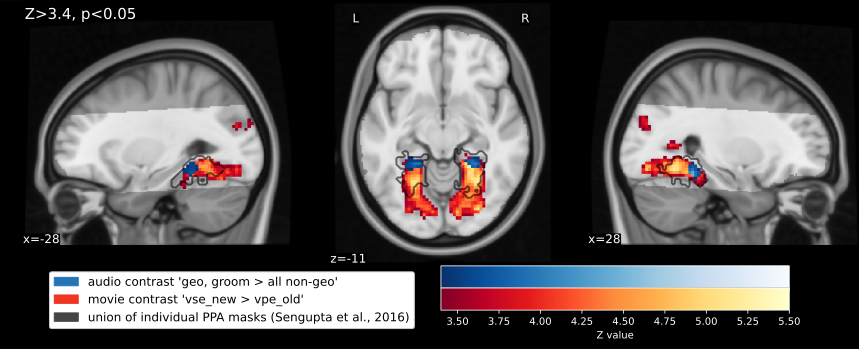
\includegraphics[width=\linewidth]{figures/group-slices}
    \caption{Mixed-effects group-level (N=14) GLM results. Significant clusters
        (Z>3.4, p<.05 cluster-corrected) are overlaid on the MNI152 T1-weighted
        head template (gray).
        Light gray: The audio-description's field-of-view
        (cf. \citep{hanke2014audiomovie}).
        Black: outline of overlapping individual PPA ROIs.
        The results of audio-description's primary $t$-contrast (blue) that
        compares geometry-related nouns to non geometry-related nouns spoken by
        the audio-description's narrator (\texttt{geo, groom > all non-geo})
        are overlaid over the movie's primary $t$-contrast (blue) that compares
        cuts to a new setting with cuts to a familiar perspective
        (\texttt{vse\_new > vpe\_old})
   \citep{sengupta2016extension}.}
    \label{fig:group-slices}
\end{figure*}

\subsubsection{AO: robustness of PPA across contrasts}

\todo[inline]{tables of significant clusters all contrasts = overkill!? Link to NeuoVault is added; sign. clusters of all contrasts are listed in the comments}

% all eight AO PPA contrasts
In order to test the robustness of our findings, we created overall eight
$t$-contrasts for the AO stimulus (see Table \ref{tab:ao-contrasts}).
% results
All contrasts except contrast 7 (\texttt{se\_new}, \texttt{se\_old} >
non-spatial categories) and contrast 8 (\texttt{se\_new} > non-spatial
categories) yielded significant bilateral clusters in anterior regions of the
group PPA overlap (see Figure \ref{fig:stability-slices}).
% statement/answer
Results suggest that our findings do not depend on one specific contrasts but
are robust across differently designed contrasts.
% question
\todo[inline]{concluding statement often feels like interpretation/discussion}
%
\todo[inline]{Discussion: discuss that contrasts make ``less and less'' sense}

% figure group results of robustness across all AO & AV contrasts
\begin{figure*} \centering
    \includegraphics[width=\linewidth]{figures/stability-slices}
    \caption{Overlap of significant clusters (Z>3.4; p<.05, cluster corrected)
        The audio-description's contrasts 1-8 (blue; \ref{tab:ao-contrasts})
        are overlaid over the audio-visual movie's contrasts 1-5 (red;
        \ref{tab:av-contrasts}) that were used to [isolate] the PPA
        Cluster are overlaid on top of the MNI152 T1-weighted head template
        (gray).
        Black: outline of overlapping individual PPA ROIs.
        Light gray: The audio-description's field-of-view (cf.
        \citep{hanke2014audiomovie}).}
    \label{fig:stability-slices}
    \end{figure*}

\paragraph{AO: other significant clusters across contrasts}
% precuneus = retrosplenial cortex ?
\todo[inline]{significant clusters in other regions than PPA could or should (?)
also be reported? Following is a short list; depends on the discussion I guess;
anyhow: clusters are not ``random'' but make sense which speaks for the use of
naturalistic stimuli}

\begin{itemize}
\item RSC (and ventral precuneus): 7 contrasts (all bilateral)
\item lateral occipiatal cortex: 6 contrasts (4 bilateral, 2 unilateral =
    transverse occipital sulcus / occipiatal place area?; AO \& AV clusters
    overlap but AO clusters are more lateral, AV cluster are more medial \&
    caudal)
\item right superior temporal gyrus (auditory cortices): 4 contrasts
\item (smallish) prefrontal clusters: 3 contrasts (non-overlapping)
\end{itemize}

\subsubsection{AV: PPA in primary contrast}
% AV intro
As conceptual/cross-modal control of the group average results, we also analyzed
data from the audio-visual movie by contrasting different kinds of movie cuts
independent(ly) from the frames' visual content following the cut.
% AV primary contrast
The movie's primary $t$-contrast that compared cuts to a setting that was not
depicted before to a recurring setting (\texttt{vse\_new > vpe\_old}) yielded
three significant clusters (see Table \ref{tab:res-av-group1}, Figure
\ref{fig:group-slices}).
% PPA (others the clusters extend into).
One cluster spans across the midline and comprises, parts of the intracalcarine
and cuneal cortex, the lingual gyrus and retrosplenial cortex, the occipital and
temporal fusiform gyrus and the parahippocampal cortex (reported from posterior
to anterior) in both hemispheres.
% LOC
Two additional homologous clusters are located in the superior lateral occipital
cortex (left bigger than right).


\begin{table*}[t]
\caption{Significant clusters (z-threshold Z>3.4; p<.05 cluster-corrected)
    of the primary $t$-contrast for the audio-visual movie comparing cuts to a
    setting that was not depicted before to a recurring setting
    (\texttt{vse\_new > vpe\_old}).
    Clusters sorted by voxel size.
    The first brain structure given contains the voxel with the maximum Z-Value,
    followed by brain structures from posterior to anterior, and partially
    covered areas (l. = left; r. = right; c. = cortex; g. = gyrus).}
\label{tab:res-av-group1}
\begin{tabular}{rrrrrrrrrp{3cm}}
\toprule
& & & \multicolumn{3}{r}{max location (MNI)} & \multicolumn{3}{r}{center of gravity (MNI)} &
\\ \cmidrule{4-6} \cmidrule{7-9}
voxels & $p_{corr.}$ & Z-max & x & y & z  & x & y & z & structure \\
\midrule
3003 & 0 & 5.31 & 22.5 & -45.5 & -12 & 4.53 & -63.3 & -3.72 & r. lingual g.; r. cuneal c., intracalcarine c., bilaterally occipital fusiform g., temporal fusiform c., posterior parahippocampal c.  \\
154 & 6.56E-07 & 4.46 & -35 & -83 & 28 & -32.8 & -86.2 & 21.4 & l. superior lateral occipital c. \\
121 & 7.69E-06 & 4.65 & 25 & -80.5 & 25.5 & 23.7 & -83.8 & 25.4 & r. superior lateral occipital cortex \\
\bottomrule
\end{tabular}
\end{table*}

\subsubsection{AV: robustness of PPA across contrasts}

% all eight AV PPA contrasts
Here again in order to test the robustness of our findings, we created four
additional $t$-contrasts for the AV stimulus (see Table \ref{tab:av-contrasts}).
%% results: PPA
All of the overall five AV contrasts yielded significant bilateral clusters that
overlap with the PPA group overlap (see Figure \ref{fig:stability-slices}).
[biggest overlap in posterior part of PPA group overlap  = temporal occipital
fusiform cortex] .
% concluding statement
Here again, we can show that results can in principle be accomplished by varying
the design of the contrasts.
% question
\todo[inline]{concluding statement = interpretation/discussion?}


\paragraph{AV: other signficant clusters across contrasts}

\begin{itemize}
\item lateral occipital cortex: 4 contrasts (all bilateral)
\end{itemize}


\subsubsection{AO \& AV: (negative) control contrasts}

\todo[inline]{for completeness, contrasts are mentioned in the method section.
Shall results be reported (and later discussed)?}

% AO stimulus
AO stimulus (using annotation of movie cuts) all null results except: contrast 9
(vse\_new > pe\_old): right RSC.
% correlation of these nouns with cuts
Compare Figure \ref{fig:reg-corr}: nouns that cue change to a new setting are
correlated  with cuts to a new setting (vse\_new; r$\approx$0.3; second highest
correlation of a verbal cue category with a cut category.

% AV stimulus
AV stimulus. All contrasts using ``no cut condition'' > XY yield null results.
The contrast that uses the narrator's nouns but in the AV stimulus (se\_new >
se\_old): right PPA, bilateral sup. lat. occ. cortex; LOC (l/r), right superior
parietal lobe. Compate Figure \ref{fig:reg-corr}: nouns that cue change to a new
setting are correlated  with cuts to a new setting (vse\_new; r$\approx$0.3;
second highest correlation of a verbal cue category with a cut category; AND:
nouns that cue change to a familiar setting are somewhat correlated with cuts to
a familiar setting (se\_old; r$\approx$0.4; highest correlation of a verbal
category with a cut category).


\subsection{individual results}

\todo[inline]{other reasons than localization performance?}

% why individual results in the first place.
We also investigated [localization performance] of both naturalistic paradigms
on the level of individual subjects.\todo{depends on ``naturalistic stimulus for
localization''}
% results in both subject and group space
Time series of all subjects were analyzed both in group space and subject space.
 space
For better comparison of results across participants, we here report results
($z$-maps; Z>3.4, p<.05 cluster-corrected) of the analyses that was performed in
group space.
% ref to figure
Figure \ref{fig:subs-thresh-ppa} depicts thresholded $z$-maps of the primary AO
and AV $t$-contrast, and the outline of the individual PPAs
\citep{sengupta2016extension} overlayed on the MNI152 template (transversal
slice z=-11 for all subjects was chosen as it depicts voxels of significant
clusters in almost all subjects).
% individual z-maps -> dataset
Results of the analyses that were performed in each subject's subject-space
(unthresholded $z$-maps and thresholded $z$-maps with Z>2.3, p<.05 cluster
corrected) can be found at
\href{https://neurovault.org/collections/KADGMGVZ/}{NeuroVault}.\todo{still
private collection} .
% report here in group

% results in detail voxels of significant clusters in PPA ROI (and  RSC
% liberally)
% sub-01 (m): PPA (l/r), AO (l/r), AV (-/r); RSC: AO (l/r), AV (-/-)
% sub-02 (m): PPA (l/r), AO (-/-), AV (l/-); RSC: AO (-/-), AV (-/-)
% sub-03 (f): PPA (l/r), AO (-/-), AV (-/r); RSC: AO (-/-), AV (-/-)
% sub-04 (f): PPA (-/r), AO (l/r), AV (-/r); RSC: AO (l/r), AV (-/-) !
% sub-05 (m): PPA (l/r), AO (-/-), AV (-/-); RSC: AO (-/-), AV (-/-)
% sub-06 (m): PPA (l/r), AO (l/r), AV (-/-); RSC: AO (l/-), AV (-/-)
% sub-09 (m): PPA (l/r), AO (l/-), AV (l/r); RSC: AO (l/r), AV (l/r)
% sub-14 (f): PPA (l/r), AO (l/r), AV (-/r); RSC: AO (l/r), AV (-/-)
% sub-15 (m): PPA (l/r), AO (l/r), AV (-/r); RSC: AO (l/r), AV (l/r)
% sub-16 (m): PPA (l/r), AO (l/r), AV (l/r); RSC: AO (l/r), AV (l/-)
% sub-17 (m): PPA (l/r), AO (l/r), AV (l/r); RSC: AO (l/r), AV (l/r)
% sub-18 (m): PPA (l/r), AO (l/r), AV (l/r); RSC: AO (l/r), AV (-/r)
% sub-19 (f): PPA (l/r), AO (l/r), AV (-/r); RSC: AO (l/r), AV (l/r)
% sub-20 (f): PPA (-/r), AO (-/-), AV (l/r); RSC: AO (-/-), AV (-/-)

% PPA ROI (Sengupta et al., 2016)
The visual localizer experiment \citep{sengupta2016extension} yielded bilateral
clusters in 12 of 14 subjects and a unilateral right clusters in two subjects
(sub-04, sub-20) that were defined as the PPA.\todo{this is probably the part
that Simon considered as/too ``en passant''}
% procedure in Sengupta
Individual PPAs were assessed by visually inspecting unthresholded $z$-maps of
three different contrasts, and setting a subjectively best fitting $z$-threshold
to define an area in the parahippocampal gyrus [and adjacent regions of the
fusiform gyrus and anterior lingual gyrus].
% AO
In the current analysis of the AO stimulus, we use the same AO (and AV) contrast
for all subjects. We find statistically significant bilateral clusters in nine
subjects, and one cluster in the left hemisphere of sub-09 that are within or
overlapping with the individual PPA.
% subj-04
In sub-04, two homologous clusters are apparent, whereas the dedicated localizer
(and AV stimulus) yielded only one cluster in the right hemisphere.
% AV
Results of the AV contrast yield homologous clusters in five subjects,
unilateral right clusters in six subjects (of which one subjects yielded a
unilateral cluster in the visual localizer), and a unilateral left cluster in
one subject.
% difference to dedicated localizer
We find homologous clusters in sub-20, whereas the dedicated visual localizer
yielded only one cluster in the right hemisphere.
% concluding statement
\todo[inline]{concluding statement that does not sound like
interpretation/discussion?}


\begin{figure*} \centering
    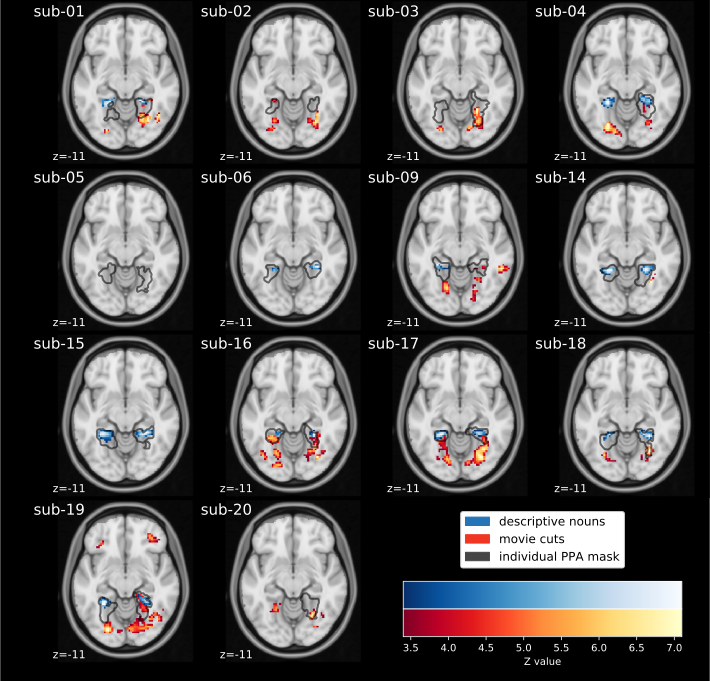
\includegraphics[width=\linewidth]{figures/subs-thresh-ppa}
    \caption{Fixed-effects individual-level GLM results (Z>3.4, p<.05
        cluster-corrected).
        Individual brains are aligned via non-linear
        transformation to a study-specific T2* group template that is
        co-registered to the MNI152 template with an affine transformation (12
        degrees of freedom).
        The results of audio-description's primary
        $t$-contrast (blue) that compares geometry-related nouns to non
        geometry-related nouns spoken by the audio-description's narrator
        (\texttt{geo, groom > all non-geo}) are overlaid over the movie's
        primary $t$-contrast (blue) that compares cuts to new setting with cuts
        to a familiar perspective (\texttt{vse\_new > vpe\_old}).
        Black:
        outline of subject-specific PPA ROIs.
        Light gray: The
        audio-description's field-of-view (cf. \citep{hanke2014audiomovie}).
        To facilitate comparisons across subjects, we chose the same horizontal
        slice (x=-11) for all subjects as this slice depicts voxels of
        significant clusters in almost all subjects.
        The figure does not show voxels of the left cluster of the AV stimulus
        in sub-09 and sub-18, and voxels of right cluster of the AV stimulus in
        sub-15.}
    \label{fig:subs-thresh-ppa}
\end{figure*}

\todo[inline]{anything else to report in the following paragraph? seems more
like just an explanation of the plots}
% Bland-Altman-Plots: why they were done
To better depict/convey the agreement and difference between individual results
of the visual localizer and the primary AO contrast, we created one
Bland-Altman-Plots for each of the 14 subjects (see Figure
\ref{fig:bland-altman}).
% x-axis
The x-axis of every subplot depicts the mean of $z$-values of two spatially
corresponding voxels taken from a subject's unthresholded $z$-map.
% y-axis
The y-axis of every subplot depicts the difference of $z$-values of two
spatially corresponding voxels (dedicated localizer minus AO stimulus).
% masking
Voxels were spatially constrained to a) voxels located in the occipital and
temporal lobes (gray; using the probabilistic Jülich Histological Atlas
\citep{eickhoff2005toolbox, eickhoff2007assignment}), b) voxels located in the
PPA overlap of all subjects (blue), and c) voxels located in individual PPA(s)
(red).
% top KDE plot
A shift of the distribution to voxels with a mean above zero can be seen the
further we constrain voxels to the individual PPA (see KDE plot for the x-axis).
% right KDE plot
Values above the horizontal line depict voxels that show a higher $z$-value in
the dedicated localizer, values below the horizontal line depict voxels that
show higher $z$-value in the AO stimulus.

\begin{figure*} \centering
    \includegraphics[scale=0.28]{figures/subjs_bland-altman.png}
    \caption{Bland-Altman-Plots for individual subjects. The x-axis depicts the
        mean of two spatially corresponding voxels in the unthresholded z-map of
        the visual localizer and in the unthresholded z-map of contrast 1 of the
        AO stimulus (KDE plot on the top). The y-axis depicts the difference of
        two voxels (KDE plot on the right).
        The overlays depict voxels spatially contrained to be located in the
        temporal and occipital cortex (gray),
        PPA overlap of all subjects (blue),
        and individual PPA(s) (red).}
    \label{fig:bland-altman} \end{figure*}


\section{Discussion}

\todo[inline]{SE: die result-synopsis noch nicht optimal. Vielleicht gehe ich
aber auch mit der falschen Perspektive ran? Für mich würde der Vergleich
"localizer vs naturalistic" im vordergrund stehen, AO vs AV dann eine sehr
spannende aber logisch nachgeschaltete Frage sein.}

\todo[inline]{SE: Bei Ergebnissen \& Diskussionen zu Stability fehlt mir
irgendwie immer der Kontext, wie sich die Kontraste denn unterschieden haben und
welche davon z.B. im Ergebnis wo von den anderen abgewichen haben. Das würde ja
wichtige Hinweise geben; COH: imo discussing that will let the paper get way out
of hand}

\todo[inline]{SE: VIS vs AV vs AO: Wer liefert was über die PPA. Dieser
Vergleich bzw. die Diskussion über Gemeinsamkeiten \& Unterschiede fehlt mir
etwas}

\todo[inline]{SE: RSC etc: Irgendwie waren die bis zu Diskussion eher ein
afterthought. Daher etwas überraschend, vielleicht in Einleitung und Results
schon mehr bringen; COH: afterthought, for sure; It was highly probable that RSC
would show up but it wasn't aim of the study (had no ROIs for it anyway); imo
this is an issue of ``nice story telling'' vs. HARKing} 

\todo[inline]{discussion explains how results fill gap identified in
intro}

\todo[inline]{provides caveats to the interpretation describes how the paper
advances the field by providing new opportunities}

\todo[inline]{typically done by recapitulating the results, discussing
limitations, and then revealing how the central contribution may catalyze future
progress}

\todo[inline]{first paragraph summarizes the important findings from the results
section, focusing on their meaning}

% previous studies: visual
Previous studies reported bilaterally increased hemodynamic activity in the PPA
when participants were watching static pictures of landscape compared to
pictures of faces or objects (e.g. \citep{epstein1998ppa,
epstein1999parahippocampal}) whereas one study using spoken sentences reported
mixed results \citep{aziz2008modulation}.
% we use similar statistical models but with naturalistic stimuli
Similarly to previous studies that used small sets of experimentally controlled
stimuli, we also used GLMs to investigate hemodynamic brain activity during two
naturalistic stimuli.
% more than just one contrast
For both naturalistic stimuli, we computed several $t$-contrasts that differed
in the contrasted categories of stimulus features and the amount of available
data to test the robustness of our findings.
% comparison to localizer experiment
We compare results of the primary contrast of each stimulus on the level of
individual subjects to results that we gained from a visual localizer experiment
done with the same subjects \citep{sengupta2016extension}.
% summary of results main finding
Results of our whole-brain analyses suggest that the perception of verbal
``spatial information'' embedded in an auditory narrative contrasted with
``non-spatial information'' is correlated with increased activation in the
anterior PPA of both hemispheres.
% to do
Other possible ``honourable'' mentions (here? and in the following discussion?)
\begin{itemize}
    \item RSC
    \item what could be LOC / OPA
    \item AV; should (shortly) be discussed
    \item robustness (imo shortly discussed; it is about robustness not about
        how all contrasts are different in detail and how results differ in
        detail; yes, totally interesting but out of scope
    \item discuss negative contrasts?
\end{itemize}

\subsection{correlation of regressors}

\todo[inline]{Following paragraph could pasted into method section to save space
here; a short interpretation is given there already; so methods/ results/
discussion are not absolutely separated there already}
% stimuli not designed for research purposes
The audio-description and the movie were not designed to be used in a BOLD fMRI
experiment but to entertain their audiences.
%
As a results, stimulus features that we annotated to create the regressors could
have been correlated leading to shared variance that lowers detection power.
% computing the correlations
Hence, we first tested for correlation of regressors within and across both
naturalistic stimuli (s. Figure \ref{fig:reg-corr})
% results of computing feature correlation
Results show no to minor correlations of regressors with regressors of the same
stimulus.
% encouraged by that we build contrasts (statement)
Thus, we felt encouraged to create traditional/canonical voxel-wise GLMs that
modeled and contrasted hemodynamic activity similarly to previous studies that
used conceptualized stimuli.


% The second through fourth paragraphs may deal with potential weaknesses
% linking it to the relevant literature or how future experiments can deal
% with these weaknesses.

% The fifth paragraph may then culminate in a description of how the paper moves
% the field forward.

% Discussion paragraphs often conclude by describing a clever, informal way of
% perceiving the contribution or by discussing future directions that can extend
% the contribution.

% step by step, the reader thus learns to put the paper’s conclusions into the
%right context.


\subsection{group level: AO \& AV (PPA only)}

\todo[inline]{I read Aziz again: visual localizer: radius of 16 mm around peak
    voxel in each hemisphere = PPA; sentence experiment: reduced activity only
    in left PPA, and only for famous places vs famous faces; I think they ran
    their f-test on the average of the PPA voxels! anyway: their analysis is
complicated, yet not sophisticated}

% AO stimulus
Group results of the AO stimulus' primary contrast yielded spatially concise
clusters in the anterior part of the PPA group overlap that we gained from a
visual localizer experiment \citep{sengupta2016extension}.
% diff to Aziz (2008)
Unlike \citep{aziz2008modulation} who modeled events from on- to offset of
sentences (describing unknown and famous places and faces), we modeled events
from on- to offset of single words (that cue the listener about the missing
visual content).
% conclusion
\citep{aziz2008modulation} found significantly increased activity in only the
left PPA and only for sentences describing famous places compared to famous
faces. Contrary, our group results suggest that auditory spatial information
compared to non-spatial information correlates with bilaterally increased
activation in its anterior.\todo{nice! and\dots?}

% tasks in previous studies
Usually studies that use small sets of experimentally controlled stimuli also
employ a task to keep subjects attentive to the stimuli.
% but epstein1998
Nevertheless, one early block-design study \citep{epstein1998ppa} compared
results from a paradigm that employed a (perceptual) judgment task of static
pictures to the same paradigm but without that task.
% results during no task
Hemodynamic activity was less but still significantly increased when
participants had no task to keep them alert and attentive to the stimuli.
% we have no task neither
Our paradigm is similar in that sense that our participants had no behavioral or
cognitive task (e.g. forming a mental image of the stimuli; cf.
\citep{ocraven2000mental})  but just had to ``enjoy the audio-description''.
% but we are still different
Our paradigm still differs from \citep{epstein1998ppa} because the modeled
stimulus features were incidentally embedded in a continuous stream of auditory
information.
% concluding statement: kinda automatic process
The lack of a task suggests that verbal spatial information is processed in the
anterior PPA in an automatic fashion and does not necessarily rely on
deliberately paying attention to verbal spatial information.
%
Further, the incidential occurrence of modeled features prevents participants
from making assumptions about the investigated perceptual process by just being
exposed to the paradigm which mimics experiencing the world outside the lab more
closely.

% AV stimulus
Group results of the AV stimulus' primary contrast yielded bilateral clusters
that span the group overlap of individual PPA ROIs from anterior to posterior.
% difference in location/size to AO and VIS
Clusters also expand into more posterior regions (occipital fusiform gyrus,
lingual gyrus, and intracalcarine cortex).\todo{which of these regions (do not
overlap) with group ROI?}
% confound of higher perception
This larger extension, especially into the primary visual cortex, can be
attributed to the fact that we averaged the content of individual frames after a
cut and did not control for confounding features like depicted faces or
objects,and low-level visual features.
% cross-modal control purpose?
\todo[inline]{better frame that it is conceptual/cross-modal control; but what
do the results tell us? yes, it ``kinda works'' but \dots?}
\todo[inline]{concluding statement regarding AV vs AO and cross-modality of
results?}


\subsection{robustness of contrasts}

% why we did a couple of contrasts
For both stimuli we created several contrasts that varied the amount of events
available for the analysis and how well the annotated events within categories
on average matched the stimulus type that we assumed to be preferentially
processed in the PPA.
% PPA AO
Regarding contrasts of the AO stimulus, six of eight contrasts show significant
bilateral clusters in the anterior part of the group PPA overlap.
% PPA AV
Regarding contrasts of the AV stimulus, all five contrasts show significant
bilateral clusters in the PPA but also extending into more posterior brain
regions.
% results indicate robustness
Thus, the results of the additional contrasts indicate that our findings are
robust across contrasts do not depend on the design of one specific
contrasts.

% but
Nevertheless, results are still influcended by [sensitive to] the amount of
available data and how well the feature space is modeled.
% example
For example, contrast 8 of the AO stimulus (\texttt{se\_new} > texttt{se\_old})
that used the most heterogeneous categories comprising the least amount of
events yielded neither a significant cluster in the right-hemispheric nor
left-hemispheric PPA.
% concluding statement
Hence, investigators using model-driven analyses have to consider how many
events a stimulus to be chosen may provide and how homogeneous the events to be
averaged might be.

% ``confounding'' clusters
Despite performing a whole brain analysis, we do not find many [random] clusters
in single contrasts or even systematically across contrasts that hamper the
interpretation of results.\todo{ouff\dots}
% AV: null results regarding attention and eye movements
For example in the AV results, we do not find significant clusters that could be
attributed to cognitive processes like attention or eye movements\todo{should
already be mentioned in disc. of primary contrasts}
% AO: auditory cortices
Nevertheless, contrasts of the AO stimulus that compare verbal cues about the
change of a setting (\texttt{se\_new} or \texttt{se\_old}) to all non-spatial
categories (cf. contrasts 2, 3, 6, 7) show significant clusters in (primary and
secondary) auditory cortices.
% averaging vs. nuisance regressors
This suggests that variance correlating with lower level auditory processes was
not averaged out across trials and nuisance regressors did not capture enough
variance.\todo{ouf\dots}
% possible reason
Significant clusters in auditory cortices could be correlating with a possible
change of the soundscape when the narrator of the audio-description (or a cut in
the movie) switches to a another setting.
% concluding statement
Thus, investigators that use model-driven methods to investigate brain functions
using naturalistic stimuli should (extensively) annotate the stimulus material
and test for correlations among variables.


\subsection{consistencies across contrasts}

\subsubsection{anterior vs. posterior PPA}

% intro
Results of the AO contrasts consistently yielded significant clusters spatially
constrained to the anterior part of the PPA group overlap [and to the anterior
part of significant clusters of the AV contrasts].
% PPA might have submodules
Previous studies provide evidence that the posterior PPA (pPPA) and anterior PPA
(aPPA) show differences in both functional connectivity profiles and in response
to low- and high-level visual features.

% posterior connectivity
The pPPA is more strongly functionally connected to the occipital visual cortex
\citep{baldassano2013differential, baldassano2016two}.
% including lateral occipital cortex (LOC) and transverse occipital sulcus (TOS)
% functionality
Moreover, the pPPA is functionally more responsive than the aPPA to low-level
features of scenes or (abstract) objects \citep{baldassano2013differential,
nasr2014thinking, rajimehr2011parahippocampal}.

% anterior
The aPPA is more strongly functionally connected to portions of the default mode
network, including caudal inferior parietal lobe (cIPL), the restrosplenial
complex (RSC), medial PFC and the lateral surface of the anterior temporal lobe
\citep{baldassano2013differential, baldassano2016two}
% anterior cIPL is defined using the Eickhoff–Zilles PGp probabilistic
% cytoarchitectonic map
Moreover, the aPPA is functionally more responsive than pPPA to high-level
features of scenes (e.g. real-word size \citep{park2015parametric}; a scene's
abstract identity/category \citep{marchette2015outside, watson2016patterns}) and
objects (e.g. spatial contextual associations \citep{aminoff2007parahippocampal,
aminoff2013role}).

\todo[inline]{the mother of total confusion: Aminoff shifts the PPA along the
    anterior-poster axis depending on the publication; in Aminoff (2007, 2013):
    anterior PPA = spatial associations, region anterior to (!) PPA =
    non-spatial associations; in Aminoff (2015): posterior PPA = spatial
associations, anterior PPA = non-spatial associations; hence: complete bullshit;
ignore Aminoff (2015) due to various reasons}

\paragraph{conclusion: subregions}

The PPA is not a functionally homogeneous area but consists of subregions that
``activate selectively to scenes'' and ``cooperate to build a complete
representation of a scene'' \citep{baldassano2013differential}.
%
Their distinct connectivity properties do suggest that each may be involved in
specific aspects of visual and cognitive processing involved in the overarching
goal of scene understanding \citep{baldassano2013differential}.

%
The fact that anterior PPA had a lower sensitivity to our abstract object
stimuli does not necessarily imply that this region does not use object
information \citep{baldassano2013differential}. Previous work has shown that PPA
responds to objects that have spatial associations [Aminoff et al. 2007], are
space-defining [Mullally and Maguire 2011], and are navigationally-relevant
[Janzen and Van Turennout 2004]. These types of responses require spatial memory
and cannot be based purely on visual features like object shape.
\citep{baldassano2013differential}.

%
[If anterior PPA is involved in processing spatial context, then space-defining
    or navigationally-relevant objects could activate anterior PPA more strongly
    than our abstract objects, which were unfamiliar and provided no sense of
    context or orientation.
%
Further experiments will be required to determine whether what type of
object-related information is used in this region
\citep{baldassano2013differential}.]


\subsubsection{retrosplenial cortex (RSC)}

\todo[inline]{check location in primary contrast and overlap across contrasts}

\todo[inline]{report numbers of contrast in AO \& AV that show sign. clusters in
RSC}

% but RSC
Apart from the PPA, we find significantly increased activity consistently across
contrast of both contrasts in the retrosplenial cortex (RSC).
% location functionally defined
As a scene-responsive region, the RSC is functionally defined and not
necessarily identical to the anatomically defined retrosplenial cortex [26]
\citep{epstein2008parahippocampal}.
% function
The RSC is strongly active during scene viewing, scene imagery [25] and mental
imagination of navigation through familiar environments [8]
\citep{epstein2008parahippocampal}.
% location
The RSC is located in the retrosplenial cortex, and posterior cingulate region,
near to the point where the calcarine sulcus joins the parietal-occipital sulcus
\citep{epstein2008parahippocampal}.
% anatomy of real RSC
The Retrosplenial cortex (BA 29 and 30) adjoins and is partially encircled by
the posterior cingulate (BA 23 and 31) [51–56]
\citep{epstein2008parahippocampal}.

% discussion of what the RSC does
interpretation cf.: \citep{vann2009what, chrastil2018heterogeneity,
silson2019posterior}
% conclusion


% baldassano2016two
\citep{baldassano2016two}: RSC appears to be most directly involved in orienting
the viewer to the structure of the environment (both within and beyond the
borders of the presented image) for the purpose of navigational planning; it
encodes both absolute location and facing direction [Vass and Epstein, 2013;
Epstein and Vass, 2014; Marchette et al., 2014], integrates across views
presented in a panoramic sequence [Park and Chun, 2009], and shows strong
familiarity effects [Epstein et al., 2007a,b] \citep{baldassano2016two}.


\subsubsection{superior lateral occipital cortex (TOC / OPA?)}

\begin{itemize}

\item Bettencourt (2013). The Role of Transverse Occipital Sulcus in Scene
Perception \item Dilks, Kanwisher (2013). The Occipital Place Area Is Causally
and Selectively Involved in Scene Perception \item Nasr (2011). Scene-selective
    cortical regions in human and nonhuman primates \item Dilks (2011).
    Mirror-image sensitivity and invariance in object \& scene processing \item
    MacEvoy and Epstein (2007). Position selectivity in scene- and
object-responsive \item Grill-Spector (2003). The neural basis of object
    perception \item Hasson (2003). Large-scale mirror-symmetry organization
    \item Nakamura (2000). Functional delineation of the human occipito-temporal
        areas \end{itemize}

%
\citep{baldassano2016two} regarding functional difference pPPA vs. OPA: The
functional distinction between pPPA and OPA is currently unclear. Previous work
has speculated about the purpose of the apparent ventral and dorsal
``duplication'' of regions sensitive to large landmarks, proposing that it may
be related to different output goals (e.g., action planning in OPA, object
recognition in pPPA)[Konkle and Caramazza, 2013], or to different input
connections (e.g., lower visual field processing in OPA, upper visual field
processing in pPPA)[Kravitz et al., 2013; Silson et al., 2015]. OPA and pPPA may
also use information from different visual eccentricities: OPA processing less
peripheral, relatively high-resolution environmental features. pPPA processing
more peripheral, large-scale geometry, and context [Baldassano et al., 2016a]
\citep{baldassano2016two}.


\subsection{negative controls and cross-modal controls}

\todo[inline]{could be mentioned in a few sentences. But above topics a far too
much still; better embed somewhere above}


\subsection{individual analyses}

An examination of these results on an individual participant basis reveals that
this pattern remains highly reliable and, therefore, does not appear to be a
by-product of group averaging across slightly offset discrete functional
subregions[aminoff2015associative].


\subsubsection{AO stimulus}

\todo[inline]{how to discuss Bland-Altman-Plots? Let's talk about that
shortly please}

\todo[inline]{in 11 subjects there are voxels of higher z-score (in the PPA ROI)
    in the AO contrast than in the contrast of the visual localizer -> should
    all be in the anterior part of the PPA ROI, i.e. the area that belongs to
    the significant cluster of the AO contrast}

\todo[inline]{shortcoming: no task to attend to spatial information}

\todo[inline]{different level of alertness during paradigms}

% intro
In order to test the audio-description's performance as a functional localizers,
we also compared the results of the audio-description's primary contrast to
results of the dedicated visualizer on the level of individual subjects.
% results of dedicated localizer
The dedicated localizer \citep{sengupta2016extension} yielded bilateral ROIs in
12 of 14 subjects and a unilateral right ROI in two subjects (sub-04, sub-20).
% in the current study
The audio-description's primary contrast yielded significant bilateral clusters
in 9 of 14 subjects (of which sub-04 shows just right-lateralized PPA ROI)  and
a unilateral significant cluster in one subject.
% conclusion
Results of our exploratory analyses suggest that a naturalistic auditory
stimulus is suitable to localize (the anterior part) of a higher-level visual
area in the majority of subjects.

% one threshold for all
Here we used a ``one threshold fits all approach`` whereas
\citep{sengupta2016extension} chose the best fitting $z$-threshold in a
subject's unthresholded $z$-maps by visual judgment and the ``best fitting''
threshold.
% one contrast for all
Moreover, we chose the same contrast to look at individual results of all
subjects.
% chose the best contrast in the future
Similarly to \citep{sengupta2016extension} that chose the ``best'' of three
alternative contrasts (strict, relaxed, or simple contrast), future studies that
aim for individual diagnostics / ROI localization should also test more than one
contrast to gain the ``best'' individual ROIs.\todo{``best'' sounds pretty
shitty}

% quote from Hanke (2014)
\citep{hanke2014audiomovie}: Compared to AV stimulus, the AO stimulus leaves a
much larger margin for inter-individual differences in imagining scenery, as
well as actors' character and personality traits, while still preserving the
time-locked presentation of information to a listener. At the same time, the AO
stimulus limits the effect of an attentional focus on the selection of a subset
of simultaneously occurring auditory events, in contrast to the selection of
different parts of the visual field.

\todo[inline]{discussion of individual differences? what do the results
suggest? Differences in alterness, attention to spatial information,
predisposition? ``capability'' to process auditory spatial information?}

\todo[inline]{individual ``preference'' to pay attention to
spatial infos (which contradicts statement above that attention is not a
prerequisite)}


\subsubsection{AV stimulus}

\todo[inline]{was not aim of the study; AV ROIs are in the plot of individual
    slices but not in the Bland-Altman-Plots}

\subsection{shortcomings in general}

\todo[inline]{Würde nicht so sehr auf Shortcomings eingehen}

\subsubsection{AO contrast}

\todo[inline]{cf. Methods: annotation \& Methods: AO copes}
% optimal stimulus type in vision
In the visual domain, landscapes and not pictures of landmarks or buildings are
considered to be the ``optimal'' stimulus type (cf. Epstein (1998, 1999, 2003,
2008).\todo{check references}
% cateogries in primary contrasts
In the current study's primary contrast, we compared verbal cues regarding
landmarks ((\texttt{geo}; often buildings or other single aspects of a whole
scene) and elements defining the geometry of a room/locale (\texttt{groom}) to
non-spatial cues.
% we did not choose se\_new and se\_old
We did not choose the categories that contained switches from one setting to
another (\texttt{se\_new} and \texttt{se\_old}) which one might assume to
contain the auditory equivalent to the ``optimal'' visual stimulus type.
% why not se\_new or se\_old
The categories \texttt{se\_new} and \texttt{se\_old} were actually
heterogeneous: they rarely contained whole and thus a vague verbal descriptions
of landscapes (e.g. ``in a football stadium'', ``Forrest is running through the
jungle'') but mostly landmarks or buildings, and also non-spatial
cues (e.g. ``Jenny as a teenager``).
% further studies
Given that humans can identify the gist of a rich visual scene within the
duration of a single fixation \citep{henderson2003human} further studies might
investigate if categories of holistic but vague verbal descriptions of
landscapes correlate with differential hemodynamic activity in the PPA compared
to more concrete spatial cues.

% future studies
Futures studies should chose a auditory narrative that better samples the
feature space correlating with the brain process to be investigated.
% future studies: stimulus material
Future studies should probably use a different narrative that models the feature
space of spatial information ``better'' (provides more events that are more
easily classified to belong to distinctive categories).

\todo[inline]{hypothesis of increased activation correlation with changes in the
    soundscape; cf. control contrasts (e.g. \texttt{vse\_new} >
    \texttt{pe\_old}).}
% foreshadowing of narrator by soundscape
Further, verbal cues are regularly forestalled by changes of the soundscape.
% arnott
\todo[inline]{e.g. arnott2008crinkling find increased activations of PPA to
sound made by objects}
% hypothesis
We hypothesize that not just semantic information but also the mere changes of a
soundscape that cues a listener about a setting's spatial layout of could
correlate with increased activity in the PPA.


\subsubsection{AV stimulus}

\todo[inline]{AV: field size decreases later in the movie; this is a confound
based on cinematography => the stimulus changes over time}

\todo[inline]{imo opening the pandora's box of the AV shortcomings especially at
the end of the paper should be kept to a minimum of text}

% focus of study
The focus of the current study was to investigate if signficantly increased
hemodynamic activity in the PPA correlates with spatial information (compared to
``non-spatial'' information) during a naturalistic auditory stimulus.
% shortcomings
Results of the AV stimulus that we ran as a conceptual control are tempered by
using different kind of movie cuts regardless of the visual content of the movie
frame after the respective cuts.
% which leads to the ``blurred'' results
Hence we got visual confounds / clusters extending in to early visual areas.
% further studies
Since the capability to isolate clusters or networks correlating with specific
perceptual (or cognitive) processes is influenced by the amount of annotated
stimulus features further studies focusing on visual perception should annotate
and model visual features of naturalistic stimuli more rigorously.
% solution
Future studies that aim to use a movie to localize different visual areas should
extensively annotate the content of frames (e.g. using the open-source solution
``Pliers'' for feature extraction from a visual naturalistic stimulus;
\citep{mcnamara2017developing}) and record the subject's visual attention via
eye-tracking.


\subsubsection{pros \& cons of natural stimuli (esp. narrative) as localizer}


\section{Conclusions}

\todo[inline]{template has no section ``conclusion'' -> use the last paragraph}

\todo[inline]{Conclusions aber irgendwie frage ich mich das relativ durchgehen):
Warum ist der Fokus so sehr auf Audiobook / AO, während AV doch eigentlich more
natural and engaging ist?}

% natural stimulation
Intro: Natural stimuli like movies \citep{hasson2008neurocinematics,
sonkusare2019naturalistic} or narratives \citep{honey2012not,
lerner2011topographic, silbert2014coupled} offer an easy to implement,
(continuous,) complex, immersive, task-free paradigm that more closely resembles
our natural dynamic environment than traditional experimental designs.
% why naturalisti stimuli are so cool
(see also \citep{sonkusare2019naturalistic, eickhoff2020towards,hamilton2018revolution})
% re-use of data for independent research question
Due to their continuity, complexity, and length, they offer a vast amount of
data on a variety of brain functions like low-level perception, attention,
comprehension, memory, emotions, or social interactions. This suggests the data
can later be reused for variety of totally different, independent research
questions, possibly on an individual level; increased compliance in individual
diagnostics in ``special'' populations where compliance is more difficult to
archive (pediatric or psychiatric)

% we annotated a couple of features to build contrasts
Method: The feature ``auditory spatial information'' is just one example of a
stimulus feature that can be annotated and used to build a model.
% data-driven vs. model-driven
Why we used a traditional GLM...

% results
Results: Our results demonstrate...

% conclusion: AO and AV robustness
In summary, our results across add further evidence that model-driven analyses
can be run on data from naturalistic stimuli to isolate brain activity
correlating with specific perceptual processes.
% but
Nevertheless isolation performance relies on how well the model captures
different aspects of the stimuli's feature space.

% conclusion auditory localizer
Conclusion: Thus, a complex but naturally engaging auditory stimulus like an
audiobook might in principle be used as a non-visual localizer for a variety of
brain functions in subjects who are not willing or able to follow task
instructions during brain scanning.


\subsection*{Code availability}
% wo kommt dieser Abschnitt hin?  how to write Code availability statement
% https://www.springernature.com/gp/authors/research-data-policy/data-availability-statements/12330880
\todo[inline]{provide supporting source code, and explaining how and where
others may access all data underlying the analysis} \emph{for all studies using
    custom code in the generation or processing of datasets, a statement must be
    included here, indicating whether and how the code can be accessed,
including any restrictions to access; include information on the versions of any
software used, if relevant, and any specific variables or parameters used to
generate, test, or process the current dataset. }

\section*{Acknowledgements}
% Text acknowledging non-author contributors. Acknowledgements should be brief, and should not include thanks to anonymous referees and editors, or effusive comments. Grant or contribution numbers may be acknowledged.
% Author contributions Please describe briefly the contributions of each author to this work on a separate line.
\emph{COH did this and that.
MH did this and that.
We are grateful to \href{www.florianschurz.de}{Florian Schurz} who initiated doing the annotation of the descriptive nouns, and performed the preliminary annotation of nouns.}

\section*{Competing financial interests}
\emph{A competing financial interests statement is required for all accepted
papers published in \emph{Scientific Data}. If none exist simply write,
``The author(s) declare no competing financial interests''.}

\section*{Figures Legends}
\emph{Figure should be referred to using a consistent numbering scheme through
the entire Data Descriptor. For initial submissions, authors may choose
to supply this document as a single PDF with embedded figures, but
separate figure image files must be provided for revisions and accepted
manuscripts. In most cases, a Data Descriptor should not contain more
than three figures, but more may be allowed when needed. We discourage
the inclusion of figures in the Supplementary Information \textendash{}
all key figures should be included here in the main Figure section.}

\emph{Figure legends begin with a brief title sentence for the whole figure
and continue with a short description of what is shown in each panel,
as well as explaining any symbols used. Legend must total no more
than 350 words, and may contain literature references.}

\section*{Tables}

\emph{Tables supporting the Data Descriptor. These can provide summary information
(sample numbers, demographics, etc.), but they should generally not
be used to present primary data (i.e. measurements). Tables containing
primary data should be submitted to an appropriate data repository.}

\emph{Tables may be provided within the \LaTeX{} document or as separate
files (tab-delimited text or Excel files). Legends, where needed,
should be included here. Generally, a Data Descriptor should have
fewer than ten Tables, but more may be allowed when needed. Tables
may be of any size, but only Tables which fit onto a single printed
page will be included in the PDF version of the article (up to a maximum
of three).}

{\small\bibliographystyle{unsrtnat}
\bibliography{references}}

%\begin{thebibliography}{1}
%\expandafter\ifx\csname url\endcsname\relax
%  \def\url#1{\texttt{#1}}\fi
%\expandafter\ifx\csname urlprefix\endcsname\relax\def\urlprefix{URL }\fi
%\providecommand{\bibinfo}[2]{#2}
%\providecommand{\eprint}[2][]{\url{#2}}
%
%\bibitem{cite1}
%\bibinfo{author}{Califano, A.}, \bibinfo{author}{Butte, A.~J.},
%  \bibinfo{author}{Friend, S.}, \bibinfo{author}{Ideker, T.} \&
%  \bibinfo{author}{Schadt, E.}
%\newblock \bibinfo{title}{{Leveraging models of cell regulation and GWAS data
%  in integrative network-based association studies}}.
%\newblock \emph{\bibinfo{journal}{Nature Genetics}}
%  \textbf{\bibinfo{volume}{44}}, \bibinfo{pages}{841--847}
%  (\bibinfo{year}{2012}).
%
%\bibitem{cite2}
%\bibinfo{author}{Wang, R.} \emph{et~al.}
%\newblock \bibinfo{title}{{PRIDE Inspector: a tool to visualize and validate MS
%  proteomics data.}}
%\newblock \emph{\bibinfo{journal}{Nature Biotechnology}}
%  \textbf{\bibinfo{volume}{30}}, \bibinfo{pages}{135--137}
%  (\bibinfo{year}{2012}).
%\end{thebibliography}

\section*{Data Citations}

Bibliographic information for the data records described in the manuscript.

1. Lastname1, Initial1., Lastname2, Initial2., ...\& LastnameN, InitialN. \emph{Repository name} Dataset accession number or DOI (YYYY).

\end{document}
\documentclass[english]{article}
